%% abtex2-modelo-trabalho-academico.tex, v-1.9.7 laurocesar
%% Copyright 2012-2018 by abnTeX2 group at http://www.abntex.net.br/ 
%%
%% This work may be distributed and/or modified under the
%% conditions of the LaTeX Project Public License, either version 1.3
%% of this license or (at your option) any later version.
%% The latest version of this license is in
%%   http://www.latex-project.org/lppl.txt
%% and version 1.3 or later is part of all distributions of LaTeX
%% version 2005/12/01 or later.
%%
%% This work has the LPPL maintenance status `maintained'.
%% 
%% The Current Maintainer of this work is the abnTeX2 team, led
%% by Lauro César Araujo. Further information are available on 
%% http://www.abntex.net.br/
%%
%% This work consists of the files abntex2-modelo-trabalho-academico.tex,
%% abntex2-modelo-include-comandos and abntex2-modelo-references.bib
%%

% ------------------------------------------------------------------------
% ------------------------------------------------------------------------
% abnTeX2: Modelo de Trabalho Academico (tese de doutorado, dissertacao de
% mestrado e trabalhos monograficos em geral) em conformidade com 
% ABNT NBR 14724:2011: Informacao e documentacao - Trabalhos academicos -
% Apresentacao
% ------------------------------------------------------------------------
% ------------------------------------------------------------------------

\documentclass[
	% -- opções da classe memoir --
	12pt,				% tamanho da fonte
	openright,			% capítulos começam em pág ímpar (insere página vazia caso preciso)
	oneside,			% para impressão em recto e verso. Oposto a oneside
	a4paper,			% tamanho do papel. 
	% -- opções da classe abntex2 --
	%chapter=TITLE,		% títulos de capítulos convertidos em letras maiúsculas
	%section=TITLE,		% títulos de seções convertidos em letras maiúsculas
	%subsection=TITLE,	% títulos de subseções convertidos em letras maiúsculas
	%subsubsection=TITLE,% títulos de subsubseções convertidos em letras maiúsculas
	% -- opções do pacote babel --
	% english,			% idioma adicional para hifenização
	% french,				% idioma adicional para hifenização
	% spanish,			% idioma adicional para hifenização
	brazil				% o último idioma é o principal do documento
	]{abntex2}

% ---
% Pacotes básicos 
% ---
\usepackage{lmodern}			% Usa a fonte Latin Modern			
\usepackage[T1]{fontenc}		% Selecao de codigos de fonte.
\usepackage[utf8]{inputenc}		% Codificacao do documento (conversão automática dos acentos)
\usepackage{indentfirst}		% Indenta o primeiro parágrafo de cada seção.
\usepackage{color}				% Controle das cores
\usepackage{graphicx}			% Inclusão de gráficos
\usepackage{microtype} 			% para melhorias de justificação
\usepackage{hyperref}
\usepackage[printonlyused]{acronym}
\usepackage{multirow}
\usepackage[table,xcdraw]{xcolor}
\usepackage{subfig}
% ---
		
% ---
% Pacotes adicionais, usados apenas no âmbito do Modelo Canônico do abnteX2
% ---
\usepackage{lipsum}				% para geração de dummy text
% ---

% ---
% Pacotes de citações
% ---
\usepackage[brazilian,hyperpageref]{backref}	 % Paginas com as citações na bibl
\usepackage[alf]{abntex2cite}	% Citações padrão ABNT

% --- 
% CONFIGURAÇÕES DE PACOTES
% --- 

% ---
% Configurações do pacote backref
% Usado sem a opção hyperpageref de backref
\renewcommand{\backrefpagesname}{Citado na(s) página(s):~}
% Texto padrão antes do número das páginas
\renewcommand{\backref}{}
% Define os textos da citação
\renewcommand*{\backrefalt}[4]{
	\ifcase #1 %
		Nenhuma citação no texto.%
	\or
		Citado na página #2.%
	\else
		Citado #1 vezes nas páginas #2.%
	\fi}%
% ---

% ---
% Informações de dados para CAPA e FOLHA DE ROSTO
% ---
\titulo{Desenvolvimento de um escalonador para \textit{Kubernetes} distribuído em microsserviços}
\autor{Leonardo Valério Anastácio}
\local{Joinville}
\data{2022}
\orientador{Dr. Guilherme Piêgas Koslovski}
\instituicao{%
  Universidade do Estado de Santa Catarina -- Udesc
  \par
  Centro de Ciências Tecnológicas
  \par
  Bacharelado em Ciência da Computação}
\tipotrabalho{Monografia}
% O preambulo deve conter o tipo do trabalho, o objetivo, 
% o nome da instituição e a área de concentração 
%\preambulo{Modelo canônico de trabalho monográfico acadêmico em conformidade com as normas ABNT apresentado à comunidade de usuários \LaTeX.}
% ---


% ---
% Configurações de aparência do PDF final

% alterando o aspecto da cor azul
\definecolor{blue}{RGB}{41,5,195}

% informações do PDF
\makeatletter
\hypersetup{
     	%pagebackref=true,
		pdftitle={\@title}, 
		pdfauthor={\@author},
    	pdfsubject={\imprimirpreambulo},
	    pdfcreator={LaTeX with abnTeX2},
		pdfkeywords={abnt}{latex}{abntex}{abntex2}{trabalho acadêmico}, 
		colorlinks=true,       		% false: boxed links; true: colored links
    	linkcolor=blue,          	% color of internal links
    	citecolor=blue,        		% color of links to bibliography
    	filecolor=magenta,      		% color of file links
		urlcolor=blue,
		bookmarksdepth=4
}
\makeatother
% --- 

% ---
% Posiciona figuras e tabelas no topo da página quando adicionadas sozinhas
% em um página em branco. Ver https://github.com/abntex/abntex2/issues/170
\makeatletter
\setlength{\@fptop}{5pt} % Set distance from top of page to first float
\makeatother
% ---

% ---
% Possibilita criação de Quadros e Lista de quadros.
% Ver https://github.com/abntex/abntex2/issues/176
%
\newcommand{\quadroname}{Quadro}
\newcommand{\listofquadrosname}{Lista de quadros}

\newfloat[chapter]{quadro}{loq}{\quadroname}
\newlistof{listofquadros}{loq}{\listofquadrosname}
\newlistentry{quadro}{loq}{0}

% configurações para atender às regras da ABNT
\setfloatadjustment{quadro}{\centering}
\counterwithout{quadro}{chapter}
\renewcommand{\cftquadroname}{\quadroname\space} 
\renewcommand*{\cftquadroaftersnum}{\hfill--\hfill}

\setfloatlocations{quadro}{hbtp} % Ver https://github.com/abntex/abntex2/issues/176
% ---

% --- 
% Espaçamentos entre linhas e parágrafos 
% --- 

% O tamanho do parágrafo é dado por:
\setlength{\parindent}{1.3cm}

% Controle do espaçamento entre um parágrafo e outro:
\setlength{\parskip}{0.2cm}  % tente também \onelineskip

% ---
% compila o indice
% ---
\makeindex
% ---

% ----
% Início do documento
% ----
\begin{document}

% Seleciona o idioma do documento (conforme pacotes do babel)
%\selectlanguage{english}
\selectlanguage{brazil}

% Retira espaço extra obsoleto entre as frases.
\frenchspacing 

% ---
% Capa
% ---
\imprimircapa
% ---

% ---
% Folha de rosto
% (o * indica que haverá a ficha bibliográfica)
% ---
\imprimirfolhaderosto*
% ---



% ---
% Inserir a ficha bibliografica
% ---

% Isto é um exemplo de Ficha Catalográfica, ou ``Dados internacionais de
% catalogação-na-publicação''. Você pode utilizar este modelo como referência. 
% Porém, provavelmente a biblioteca da sua universidade lhe fornecerá um PDF
% com a ficha catalográfica definitiva após a defesa do trabalho. Quando estiver
% com o documento, salve-o como PDF no diretório do seu projeto e substitua todo
% o conteúdo de implementação deste arquivo pelo comando abaixo:
%
% \begin{fichacatalografica}
%     \includepdf{fig_ficha_catalografica.pdf}
% \end{fichacatalografica}

% \begin{fichacatalografica}
%	\sffamily
%	\vspace*{\fill}					% Posição vertical
%	\begin{center}					% Minipage Centralizado
%	\fbox{\begin{minipage}[c][8cm]{13.5cm}		% Largura
%	\small
%	\imprimirautor
%	%Sobrenome, Nome do autor
%	
%	\hspace{0.5cm} \imprimirtitulo  / \imprimirautor. --
%	\imprimirlocal, \imprimirdata-
%	
%	\hspace{0.5cm} \thelastpage p. : il. (algumas color.) ; 30 cm.\\
%	
%	\hspace{0.5cm} \imprimirorientadorRotulo~\imprimirorientador\\
%	
%	\hspace{0.5cm}
%	\parbox[t]{\textwidth}{\imprimirtipotrabalho~--~\imprimirinstituicao,
%	\imprimirdata.}\\
%	
%	\hspace{0.5cm}
%		1. Palavra-chave1.
%		2. Palavra-chave2.
%		2. Palavra-chave3.
%		I. Orientador.
%		II. Universidade xxx.
%		III. Faculdade de xxx.
%		IV. Título 			
%	\end{minipage}}
%	\end{center}
%\end{fichacatalografica}
% ---

% ---
% Inserir folha de aprovação
% ---

% Isto é um exemplo de Folha de aprovação, elemento obrigatório da NBR
% 14724/2011 (seção 4.2.1.3). Você pode utilizar este modelo até a aprovação
% do trabalho. Após isso, substitua todo o conteúdo deste arquivo por uma
% imagem da página assinada pela banca com o comando abaixo:
%
% \begin{folhadeaprovacao}
% \includepdf{folhadeaprovacao_final.pdf}
% \end{folhadeaprovacao}
%
\begin{folhadeaprovacao}

  \begin{center}
    {\ABNTEXchapterfont\large\imprimirautor}

    \vspace*{\fill}\vspace*{\fill}
    \begin{center}
      \ABNTEXchapterfont\bfseries\Large\imprimirtitulo
    \end{center}
    \vspace*{\fill}
    
    \hspace{.45\textwidth}
    \begin{minipage}{.5\textwidth}
        \imprimirpreambulo
    \end{minipage}%
    \vspace*{\fill}
   \end{center}
        
   Trabalho aprovado. \imprimirlocal, -- de -------- de ----

   \assinatura{\textbf{\imprimirorientador} \\ Orientador} 
   \assinatura{\textbf{Dr. Maurício Aronne Pillon} \\ Membro Banca Examinadora}
   \assinatura{\textbf{Dr. Rafael Rodrigues Obelheiro} \\ Membro Banca Examinadora}
   %\assinatura{\textbf{Professor} \\ Convidado 3}
   %\assinatura{\textbf{Professor} \\ Convidado 4}
      
   \begin{center}
    \vspace*{0.5cm}
    {\large\imprimirlocal}
    \par
    {\large\imprimirdata}
    \vspace*{1cm}
  \end{center}
  
\end{folhadeaprovacao}
% ---

% ---
% Dedicatória
% ---
% \begin{dedicatoria}
%   \vspace*{\fill}
%   \centering
%   \noindent
%   \textit{ Este trabalho é dedicado às crianças adultas que,\\
%   quando pequenas, sonharam em se tornar cientistas.} \vspace*{\fill}
% \end{dedicatoria}
% ---

% ---
% Agradecimentos
% ---
% \begin{agradecimentos}
% Os agradecimentos principais são direcionados à Gerald Weber, Miguel Frasson,
% Leslie H. Watter, Bruno Parente Lima, Flávio de Vasconcellos Corrêa, Otavio Real
% Salvador, Renato Machnievscz\footnote{Os nomes dos integrantes do primeiro
% projeto abn\TeX\ foram extraídos de
% \url{http://codigolivre.org.br/projects/abntex/}} e todos aqueles que
% contribuíram para que a produção de trabalhos acadêmicos conforme
% as normas ABNT com \LaTeX\ fosse possível.
% Agradecimentos especiais são direcionados ao Centro de Pesquisa em Arquitetura
% da Informação\footnote{\url{http://www.cpai.unb.br/}} da Universidade de
% Brasília (CPAI), ao grupo de usuários
% \emph{latex-br}\footnote{\url{http://groups.google.com/group/latex-br}} e aos
% novos voluntários do grupo
% \emph{\abnTeX}\footnote{\url{http://groups.google.com/group/abntex2} e
% \url{http://www.abntex.net.br/}}~que contribuíram e que ainda
% contribuirão para a evolução do \abnTeX.
%
% \end{agradecimentos}
% ---

% ---
% Epígrafe
% ---
% \begin{epigrafe}
%    \vspace*{\fill}
%	\begin{flushright}
%		\textit{``Não vos amoldeis às estruturas deste mundo, \\
%		mas transformai-vos pela renovação da mente, \\
%		a fim de distinguir qual é a vontade de Deus: \\
%		o que é bom, o que Lhe é agradável, o que é perfeito.\\
%		(Bíblia Sagrada, Romanos 12, 2)}
%	\end{flushright}
%\end{epigrafe}
% ---

% ---
% RESUMOS
% ---
% resumo em português
\setlength{\absparsep}{18pt} % ajusta o espaçamento dos parágrafos do resumo
\begin{resumo}
    Na contemporaneidade, nota-se uma tendência no desenvolvimento de sistemas distribuídos, a qual é impulsionada pela conteinerização de microsserviços provisionados em \textit{data centers}. Especificamente, contêiner é uma tecnologia responsável por encapsular o ambiente da aplicação abstraindo particularidades de sistema operacional, bibliotecas e configurações. Em plataformas de computação atuais (\textit{e.g.}, \textit{data centers}, nuvem) essa tecnologia é implantada em larga escala, pois o contêiner empacota aplicações com o objetivo de otimizar o uso de recurso computacional da máquina hospedeira. O \textit{Kubernetes} é um orquestrador de contêineres responsável por criar, gerenciar e escalar microsserviços na forma de contêineres. O escalonador padrão do \textit{Kubernetes} atua apenas nas estratégias de espalhamento ou agrupamento de contêineres. Para reparar essa limitação, na literatura encontram-se técnicas de escalonamento que refletem em redução de consumo energético, uso total de recursos ou equidade entre usuários. Entretanto, grande parte desses estudos não consideram o desenvolvimento de um algoritmo escalável. O escalonador baseado em arquitetura distribuída fornece otimização do uso dos recursos do \textit{data center}, como também, melhor tolerância a falhas, por consequência, diminuição considerável do tempo de espera de escalonamento em cenário de falhas. Dessa forma, o presente trabalho visou o desenvolvimento de um escalonador distribuído baseado em microsserviços para \textit{Kubernetes}, a partir do resultados observou-se um bom desempenho da proposta quando comparado com a abordagem padrão de escalonamento do \textit{Kubernetes}.
    
    \textbf{Palavras-chave}: Sistemas distribuídos, microsserviços, contêiner, \textit{Kubernetes}, escalonamento.
\end{resumo}

% resumo em inglês
\begin{resumo}[Abstract]
 \begin{otherlanguage*}{english}
   Nowdays there is a tendency in the development of distributed systems, which is driven by the containerization of microservices provisioned in data centers. Specifically, container is a technology that encapsulate the application environment, abstract particularities of the operating system, libraries and configurations. In actual computing platforms (\textit{e.g.}, data centers, cloud) this technology is deployed on a large scale, because the container packages applications with the aim of optimizing the use of the host machine's computational resources. The \textit{Kubernetes} is a container orchestrator responsible for creating, managing and scaling microservices represented by containers. The default scheduler of \textit{Kubernetes} only works on spreading or container binpacking strategies. In the literature there are scheduling techniques that reflect in energy consumption reduction, total use of resources or equity between users. But, most of these studies do not consider the development of a scalable algorithm. The scheduler based on distributed architecture provides optimization at the use of \textit{data center} resources, better fault tolerance, consequently, a considerable reduction in the scheduling waiting time in a failure scenario. Therefore, this study aims to develop a distributed scheduler based on microservices for \textit{Kubernetes}, thus increasing scalability and reducing scheduling waiting time and \textit{makespan} metrics.
   \vspace{\onelineskip}
 
   \noindent 
   \textbf{Keywords}: Distributed Systems, microservices, container, \textit{Kubernetes}, scheduling.
 \end{otherlanguage*}
\end{resumo}
% ---
% ---

% ---
% inserir lista de ilustrações, quadros e tabelas
% ---
% ---
% inserir lista de ilustrações
% ---
\pdfbookmark[0]{\listfigurename}{lof}
\listoffigures*
\cleardoublepage
% ---

% ---
% inserir lista de quadros
% ---
% \pdfbookmark[0]{\listofquadrosname}{loq}
% \listofquadros*
% \cleardoublepage
% ---

% ---
% inserir lista de tabelas
% ---
% \pdfbookmark[0]{\listtablename}{lot}
% \listoftables*
% \cleardoublepage
% ---

% ---
% inserir lista de abreviaturas e siglas
% ---
% ---
% inserir lista de abreviaturas e siglas
% ---
\pretextualchapter{\listadesiglasname}
\begin{acronym}[RWTH Aachen ]
    \large
	\acro{DC}[Dc]{\it Data center}
	\acro{DDD}[\textit{DDD}]{\textit{Design} orientado a domínio}
	\acro{HPC}[HPC]{\textit{High Performance Computing}}
	\acro{HTTP}[\textit{HTTP}]{Protocolo de Transferência de Hipertexto}
	\acro{IAAS}[\textit{IaaS}]{Infraestrutura como um Serviço}
	\acro{K8}[k8's]{\textit{Kubernetes}}
	\acro{PAAS}[\textit{PaaS}]{Plataforma como um Serviço}
	\acro{QOS}[\textit{QoS}]{\textit{Quality-of-Service}}
	\acro{RPC}[\textit{RPC}]{Protocolo de Chamada de Procedimento Remoto}
	\acro{SAAS}[\textit{SaaS}]{Software como um Serviço}
	\acro{SO}[\textit{SO}]{Sistema Operacional}
	\acro{TCC}[TCC]{Trabalho de Conclusão de Curso}
	\acro{UDESC}[UDESC]{Universidade do Estado de Santa Catarina}
	\acro{VM}[\textit{MV's}]{Máquinas virtuais}
	\acro{WWW}[\textit{WWW}]{\textit{World Wide Web}}
	\acro{KMS}[\textit{KMS}]{\textit{Kubernetes Micro Scheduler}}
\end{acronym}
\cleardoublepage
% ---
% ---

% ---
% inserir o sumario
% ---
\pdfbookmark[0]{\contentsname}{toc}
\tableofcontents*
\cleardoublepage
% ---



% ----------------------------------------------------------
% ELEMENTOS TEXTUAIS
% ----------------------------------------------------------
\textual

% ----------------------------------------------------------
% Introdução (exemplo de capítulo sem numeração, mas presente no Sumário)
% ----------------------------------------------------------
\chapter{Introdução}
Na contemporaneidade nota-se uma tendência das organizações em mover aplicações de escala corporativa para a Computação em Nuvem. As razões para essa ocorrência são múltiplas: alta disponibilidade e redundância, escala automática, gerenciamento integrado de \textit{data center} e fluxo de desenvolvimento \cite{Fritzsch}. Impulsionado pelo paradigma imposto pela Computação em Nuvem, a forma de arquitetar, testar, e implantar \textit{software} mudou fundamentalmente, de forma que aplicações escaláveis migram de monolíticas para distribuída em microsserviços, para se enquadrar na Computação em Nuvem.

O termo microsserviço surgiu nos últimos anos para descrever um método específico de arquitetar \textit{software} como um conjunto de serviços que são escalados e implementados independentemente \cite{FowlerMicrosservice}. No contexto de Nuvem Computacional, os microsserviços podem ser utilizados na forma de contêineres, que são unidades de \textit{software} autônomas que encapsulam aplicações e todas suas dependências. No contêiner, os recursos de um nó computacional são compartilhados sem a necessidade da instalação e configuração de dependências. Isso permite que os provedores de estrutura virtual instanciem, realoquem e otimizem suas aplicações de forma mais flexível com desempenho virtual próximo ao \textit{bare metal}. Além de todos esses benefícios, os contêineres oferecem isolamento a nível de sistema operacional, assim, no ponto de vista do usuário, o contêiner executa um sistema operacional independente \cite{Fazio2016, Assuno}. 

A virtualização de contêineres baseada no sistema operacional GNU/Linux é a mais popular, sendo denominada de \textit{Linux container virtualization} (LCV). Gerenciadores LCV encontrados na atualidade são \textit{Docker}, \textit{Linux Containers} (LXC) e \textit{OpenVZ} \cite{Fazio2016}. Entre os \textit{softwares} de virtualização de microsserviços baseados em contêineres, destaca-se \textit{Docker}. Essa tecnologia proporciona funcionalidades além da capacidade de virtualização, pois facilita o processo de criação, construção e controle de versão de imagens de contêineres \cite{Redhat}.
%
Existem ferramentas que gerenciam e coordenam o escalonamento de contêineres em \textit{clusters}. Para a administração de contêineres \textit{Docker} é comum o uso de tecnologias como \textit{Docker Swarm} e \ac{K8}. Ao utilizar essas ferramentas, o usuário possuirá controle da infraestrutura de maneira simplificada e será capaz de criar, alterar e remover contêineres de forma eficiente. De acordo com \citeonline{Rodriguez2018}, tecnologias como \textit{Docker Swarm} e \textit{Kubernetes} são classificados como orquestradores de contêineres. Os orquestradores atuais, além de oferecer estrutura de controle do ambiente de virtualização, também são responsáveis pelo escalonamento, replicação e alta disponibilidade das aplicações. 

Para \citeonline{Arundel}, o \textit{Kubernetes} é considerado o Sistema Operacional das Nuvens Computacionais, sendo o sistema de orquestração de contêineres padrão no mercado. Para isso, o \textit{Kubernetes} oferece um ambiente robusto para implantação de sistemas voltados para Nuvem. As principais características do orquestrador são: escala automática de cargas de trabalho, balanceamento de carga, escalonamento por agrupamento ou espalhamento, e monitoramento do \textit{cluster}.
%
O \textit{Kubernetes} é um sistema de orquestração que agrupa contêineres em \textit{pods}. \textit{Pod} é um grupo com um ou mais contêineres que compartilham recursos de armazenamento e rede. Dessa forma, contêineres dispostos em um mesmo \textit{pod} são escalonados e executados simultaneamente \cite{Google}. Ou seja, todas as dependências que a aplicação conteinerizada necessita serão lançadas e agrupadas ao mesmo tempo e \textit{pod}, respectivamente. Além disso, a \textit{Google} disponibiliza, de forma oficial, bibliotecas que utilizam \textit{Application Programming Interface} (API) do \textit{cluster} \textit{Kubernetes}  para as principais linguagens de programação (\textit{e.g.}, \textit{.NET}, \textit{Python}, \textit{Java}, \textit{Go}, \textit{JavaScript}, \textit{Haskell}). Por meio da API é possível obter o estado do \textit{cluster}, configurar, lançar e escalonar \textit{pods} \textit{Kubernetes} \cite{KubernetesAPI}.

Para realizar o escalonamento dos \textit{pods}, o \textit{kube-scheduler} executa um fluxo de operações que são separadas em duas categorias, sendo elas, filtragem e ranqueamento. Em resumo, a filtragem consiste em investigar \textit{nodes} que são capazes de executar o \textit{pod} a ser escalonado, ou seja, nessa etapa há a seleção dos \textit{nodes} do \textit{cluster} que satisfazem a solicitação de recursos do \textit{pod}. O ranqueamento, por sua vez, classifica os \textit{nodes} eleitos pela filtragem e seleciona o \textit{node} que obter a maior pontuação de acordo a solicitação de recursos do \textit{pod} \cite{Kubescheduler}.

A principal limitação do \textit{Kube-scheduler} é na etapa anterior à filtragem: o \textit{Kubernetes} utiliza um método ingênuo na escolha do próximo contêiner a ser escalonado, que consiste em escalonar de acordo com a ordem de chegada. Essa técnica também é conhecida como \textit{First-Come-First-Serverd} (FCFS) ou \textit{First-In-First-Out} (FIFO)~\cite{Ye2007}. A limitação do \textit{Kube-scheduler}, na utilização do \textit{FCFS}, reflete diretamente na escalabilidade do problema, que por consequência, degrada o \textit{makespan} (tempo total) e tempo de espera de escalonamento. Alguns motivos são elencados para defender a escolha do \textit{FCFS}, por exemplo, garantia da ausência de inanição e simples implementação algorítmica. Embora exista o consenso que há espaço de melhoria algorítmica, substituir essa técnica de escalonamento por um algoritmo refinado é uma tarefa complexa \cite{CarastanSantos2019}.

Para o desenvolvimento de uma arquitetura distribuída de escalonamento há a necessidade de elencar algumas métricas para validação da abordagem. O presente trabalho considerou de forma primordial duas métricas relacionadas com o desempenho de escalonamento: tempo de espera de escalonamento e \textit{makespan}. O tempo de espera, como a denominação sugere, é o tempo decorrido do contêiner na fila de espera até ser escalonado, considerado um \textit{delay} do momento em que o contêiner foi submetido à plataforma até sua execução. O \textit{makespan}, uma métrica diretamente proporcional ao tempo de espera, reflete no tempo total que o contêiner permaneceu na plataforma, ou seja, do momento em que foi submetido até a sua finalização. Além dessas duas métricas será analisado o comportamento do \textit{slowdown} na arquitetura distribuída proposta. O propósito do \textit{slowdown} é estabelecer proporção entre tempo de espera de um trabalho em relação ao seu tempo de processamento. As métricas aqui apresentadas, de forma resumida, são melhor exploradas na Seção 2.4.1.

\section{Objetivos}
\label{obj}

\subsection{Objetivo geral}
\label{objgeral}

Os objetivos gerais deste trabalho refletiram no desenvolvimento de um escalonador distribuído para \textit{Kubernetes}, utilização da abordagem de microsserviços na implementação e validação da abordagem diante as métricas de otimização: tempo de espera de escalonamento e \textit{makespan}.

\subsection{Objetivos específicos}
\label{objesp}

\begin{itemize}
    \item Compreender \textit{Kubernetes};
    \item Revisar escalonamento descentralizado (utilizando particionamento e duplicação de trabalho);
    \item Revisar orquestração de contêineres;
    \item Revisar arquitetura de microsserviços;
    \item Desenvolver um escalonador distribuído baseado em microsserviços;
    \item Analisar o desempenho do escalonador proposto em relação ao tempo de espera e \textit{makespan}; e
    \item Analisar o comportamento do \textit{slowdown} em arquitetura distribuída.
\end{itemize}

\newpage
\subsection{Organização do texto}

O presente trabalho está organizado a partir da seguinte estrutura: o Capítulo 2 aborda uma revisão de literatura acerca do tema proposto, desde revisão de Computação em Nuvem até alcançar as especificidades do projeto revisando \textit{Kubernetes}, microsserviços e escalonamento de tarefas. Ao fim do Capítulo 2 são apresentados os trabalhos relacionados sobre escalonamento de contêineres com diferentes objetivos. No Capítulo 3 é detalhado a proposta distribuída, ao passo que o Capítulo 4 refere-se ao plano de teste do trabalho proposto. No capítulo 5 será feita análise dos resultados coletados de acordo com o plano de testes. Por fim, o Capítulo 6 conclui o presente trabalho de conclusão de curso e abre discussão para melhorias futuras. 
% ----------------------------------------------------------

% ----------------------------------------------------------
% Revisão de literatura
% ----------------------------------------------------------
\chapter{Revisão de Literatura}
Este capítulo aborda os conceitos fundamentais relacionados ao presente trabalho. Na Seção 2.1
é apresentada os principais conceitos referentes a virtualização baseada em contêineres, em seguida, na Seção 2.2 é realizada uma revisão sobre os componentes principais do \textit{Kubernetes}. Logo, na Seção é 2.3, é introduzido o tema microsserviços, por fim, na Seção 2.4 é apresentada uma revisão acerca do tema escalonamento de tarefas.

\section {Computação em Nuvem}
Há muitas definições formais para o termo Computação em Nuvem. A definição internacionalmente aceita pelo \textit{NIST} (\textit{National Institute of Standards and Technology})\cite{mell2011nist} visa o acesso compartilhado, isolado e sob-demanda para um ambiente de recursos computacionais (\textit{e.g.}, redes, servidores, discos, aplicações e serviços). Nesse contexto, os recursos de computação são agrupados e isolados para atender multiusuários. Ou seja, usuários isolados que compartilham recursos computacionais, os quais são dinamicamente provisionados conforme a demanda. Nesse formato há a exigência de rápido ajuste de acordo com a necessidade de recursos \cite{Bersten2014}.

\subsection{Virtualização e Nuvem}
A virtualização é considerada uma técnica que permite criar ambientes simulados a partir de um único sistema, seja ele físico ou não. Dessa forma, classifica-se virtualização como tecnologia, enquanto que Nuvem como um ambiente, conjunto de recursos computacionais gerenciável, que, pode ou não, manipular virtualização \cite{Redhat-virtualization-vs-cloud}. Nos dias atuais, a virtualização de recursos é um dos pontos chaves das Nuvens modernas, a partir da virtualização as Nuvens são capazes de gerenciar ambientes elásticos, que compartilham recursos computacionais isolados logicamente \cite{Zhang2010}. Portanto, Virtualização e Nuvem não são sinônimos.

A virtualização convencional é a baseada na execução de um \textit{hipervisor} no topo de uma máquina física. Um \textit{hipervisor} é um software que cria e executa \ac{VM}. Ao utilizar \textit{hipervisor} o administrador é capaz de otimizar o uso de recursos físicos e modular partes individuais da infraestrutura no formato de \ac{VM}. Assim, os recursos são consumidos com mais eficiência na arquitetura \textit{hipervisor} quando comparado com implantações \textit{bare-metal} (direto em \textit{hardware}). Em contrapartida, apesar da otimização em relação ao \textit{bare-metal}, o \textit{hipervisor} executa múltiplos \textit{kernels} em uma única máquina física, tornando custoso o isolamento das aplicações e processos \cite{scheepers2014virtualization}.

O presente trabalho não realizará revisão completa sobre virtualização em nuvem, uma vez que na literatura são encontrado diversos trabalhos exploratórios acerca do assunto \cite{Assuno}, \cite{lu2014cloud}, \cite{aceto2013cloud}

\subsection{Contêineres}
Na contemporaneidade, os contêineres são considerados a abordagem padrão para executar cargas de trabalho. No contexto do presente trabalho, um contêiner reflete em uma unidade computacional, que é responsável por executar as aplicações. Para gerenciamento de contêineres existem diferentes orquestradores, como por exemplo, \textit{Kubernetes} e \textit{docker swarm}.

Um contêiner compreende em um conjunto de um ou mais processos dispostos de forma isolada do \ac{SO} hospedeiro. Todas dependências que são necessárias para execução do contêiner são fornecidos por uma imagem distinta. Para a maioria dos motores de contêineres, a imagem representa os passos necessários para construção de um contêiner. A virtualização baseada em contêineres (conteinerização) é considerada uma solução portável, pois permite executar o mesmo contêiner em implantações distintas. Portanto, os contêineres são ideais para encapsular aplicações, migrá-las para hospedeiros distintos sem maiores impasses, e implantar em Nuvem \citeonline{Redhat-lxc}.

Na literatura há diversas comparações entre contêineres e \ac{VM}, como desempenho, uso de recursos e segurança. O contêiner é um processo que utiliza o mesmo \textit{kernel} que o \ac{SO} hospedeiro. Já a \ac{VM} simula um \ac{SO} pleno. Outro ponto a destacar, por convenção, o tamanho de um contêiner é mensurado em \textit{megabytes}, já a \ac{VM} em \textit{gigabyte}. Além disso, nota-se uma tendência de utilizar contêineres para construção de sistemas baseado em microsserviços. Os principais fatores para essa associação é que os contêineres se enquadram no fluxo de desenvolvimento e implantação em Nuvem, são mais leves, e possuem tempo de construção e inicialização inferiores as tradicionais \ac{VM}.

Tanto a conteinerização quanto a virtualização por \textit{hipervisor} são soluções utilizadas para a implantação de \ac{SAAS} em Nuvem. Entretanto, ao passar do tempo, a conteinerização se tornará um padrão para construção de \ac{SAAS} com características escaláveis, já as \ac{VM} irão continuar com papel importante no provisionamento de \ac{SO} sob-demanda e no fornecimento de \ac{PAAS}.

As tecnologias de conteinerização são consideradas um ecossistema que fornecem ferramentas para a conteinerização. Esse ecossistema é composto por Contêiner de Aplicação, Contêiner de Sistema, Gerenciador de Contêiner e Orquestrador de Contêineres. Nessa seção serão explanados os dois primeiros sistemas, enquanto que Orquestrador de contêineres será explicado na seção \textit{Kubernetes}.

\subsection{Contêiner de Aplicação e Contêiner de Sistema}
Apesar de se basearem nas mesmas tecnologias e conceitos, há uma diferença clara entre Contêiner de Aplicação e Contêiner de Sistema, e está relacionada ao seu uso. Contêiner de Sistema visa a execução de um \ac{SO} completo, e o Contêiner de Aplicação é designado à implantação de uma aplicação ou de um componente de uma aplicação \newline \citeonline{casalicchio2020state}. Contêiner de Aplicação refere-se a um contêiner cujo único encargo é executar uma única aplicação dentro de um ambiente isolado. Entretanto, há a possibilidade de utilizar Contêiner de Aplicação como Contêiner de Sistema, mas esse comportamento não está de acordo com \textit{Docker development guidelines and best practices} \cite{berg2016guidelines}. Pois Contêiner de Aplicação são designados para executar aplicações no formato de microsserviços. Diferente dos Contêiner de Sistema que são projetados para, em nível de comparação, executar um \ac{SO} de forma similar as \ac{VM}. Um exemplo de Contêiner de Aplicação é o \textit{docker}, um exemplo de Contêiner de Sistema é o \textit{Linux Containers (LXD)}.

%%\subsection{\textit{Docker}}

%%Segundo \cite{Redhat}, o \textit{Docker} se resume em conjunto de tecnologias, as quais incluem projetos \textit{Open Source}, ferramentas que resultaram desses projeto, e a empresa \textit{Docker Inc}. Em resumo, o termo \textit{Docker} é uma ferramenta de conteinerização para gerenciamento, criação e uso de contêineres \textit{Linux}. Com o \textit{Docker} é possível provisionar contêineres como fossem aplicações isoladas elásticas e extremamente leves.

%%Docker é uma plataforma de código aberto, desenvolvido na linguagen \textit{Go} pela \textit{Google}. 

\subsection{Gerenciadores de Contêiner de Aplicação}
O Gerenciador de Contêiner de Aplicação é considerado um \textit{framework} que fornece ferramentas que auxiliam no gerenciamento de todo o ciclo de vida do contêiner. O ciclo de vida de um contêiner, desde o desenvolvimento até execução em ambiente de produção, de acordo com \textit{IBM} \cite{ibm-ciclo}, compreende em:

\subparagraph{Obtenção:}
Aquisição da imagem do contêiner. Essa etapa é considerada o ponto inicial para a criação de um novo contêiner. Em contêineres \textit{docker} há a concepção de camadas de imagens, significa que uma imagem pode ser derivada de outras imagens. Além disso, a imagem pode ser limpa, reflexo direto do \textit{kernel}.
\subparagraph{Construção:}
Em \textit{docker} há um arquivo de definição chamado \textit{Dockerfile}, nele é definido todas as dependências e a maneira que a aplicação será executada. Normalmente em um arquivo \textit{Dockerfile} há a escolha da imagem base, passos para montagem do contêiner, e um ponto de entrada para execução de um processo, comumente são utilizados processos em segundo plano. Para que ocorra a construção do contêiner com sucesso, todos os passos de montagem devem ser executados com êxito.
\subparagraph{Entrega:}
Esse passo é referente a forma que será concebida a entrega da imagem do contêiner, já construído, para o ambiente de produção.
\subparagraph{Implantação:}
Consiste na implantação da imagem do contêiner em ambiente de  produção. Ou seja, essa etapa envolve todos os passos necessários para que uma nova imagem seja implantada no ambiente de produção.
\subparagraph{Execução:}
Nessa etapa é definido o ambiente de execução do contêiner, que pode envolver: dimensionamento da aplicação por meio de réplicas, verificação de falhas e conexão com outros serviços e réplicas.

\subparagraph{Gerenciamento:}
O passo final refere-se ao gerenciamento da aplicação conteinerizada em ambiente de produção. Nessa fase, a aplicação pode estar em execução ou em suspensão. Em gerenciamento, comportamento da aplicação é monitorada, o sistema deve ser capaz de gerenciar as falhas nos contêineres que estão em execução, por exemplo, forçando a reinicialização. Enquanto que a suspensão é um estado para depuração da aplicação, com o objetivo de encontrar a origem da falha. Posteriormente, o processo passa por todas as fases novamente, iniciando em Obtenção.

Gerenciadores de Contêineres são classificados em auto-hospedados ou baseados em soluções gerenciadas. Soluções auto-hospedadas percorrem todo o ciclo de implementação de um Gerenciador de Contêiner de Aplicação: instalação, configuração e gerenciamento em \textit{datacenters} privados, máquinas virtuais ou até mesmo em \textit{clouds} geograficamente distribuídas. Por outro lado, soluções gerenciadas são ofertados por provedores de nuvem e necessitam apenas de configuração parcial \cite{casalicchio2020state}. Assim, as plataformas de conteinerização \textit{docker, LXD, OpenVZ} podem ser configuradas da mesma maneira que Gerenciadores de Contêiner de Aplicação, portanto, são exemplos de soluções auto-hospedas. Os exemplos mais populares de soluções gerenciadas são das empresas \textit{Google} e \textit{Amazon} que possuem serviços como, respectivamente, \textit{GKE} (\textit{Google Kubernetes Engine}) e \textit{EKS} (\textit{Elastic Kubernetes Service}).

\section{\textit{Kubernetes}}
Para \citeonline{Arundel}, o \textit{Kubernetes} é considerado o Sistema Operacional das Nuvens Computacionais, sendo o sistema de orquestração de contêineres padrão no mercado. Para isso, o \textit{Kubernetes} oferece um ambiente robusto para implantação de sistemas voltados para nuvem. As principais características do orquestrador são: escala automática de cargas de trabalho por meio de replicação serviço, balanceamento de carga, escalonamento por agrupamento ou espalhamento, e monitoramento do \textit{cluster}.

O \textit{Kubernetes} é um sistema de orquestração que agrupa contêineres em \textit{pods}. \textit{Pod} é um grupo com um ou mais contêineres que compartilham recursos de armazenamento e rede. Dessa forma, contêineres dispostos em um mesmo \textit{pod} são escalonados e executados juntos \cite{Google}. Ou seja, todas as dependências que a aplicação conteinerizada necessita serão lançadas e agrupadas ao mesmo tempo e \textit{pod}, respectivamente. Além disso, a \textit{Google} disponibiliza, de forma oficial, bibliotecas que utilizam API \textit{(Application Programming Interface)} do \textit{cluster} \textit{Kubernetes}  para as principais linguagens de programação (\textit{e.g.}, \textit{.NET}, \textit{Python}, \textit{Java}, \textit{Go}, \textit{JavaScript}, \textit{Haskell}). Por meio da API é possível obter o estado do \textit{cluster}, configurar, lançar e escalonar \textit{pods} no \textit{Kubernetes} \cite{KubernetesAPI}.

\subsection{Componentes \textit{Kubernetes}}
Um \textit{cluster} \textit{Kubernetes} consiste em um conjunto de servidores, chamados de \textit{nodes}, que executam serviços conteinerizados. O sistema principal do \textit{Kubernetes} é o \textit{Control Plane}, que é responsável por tomada de decisões, escalonamento e controle do estado do \textit{cluster}. O \textit{Control Plane} reside em um \textit{node} específico denominado \textit{Master} e consiste em cinco componentes:

\begin{itemize}
    \item \textit{Kube-apiserver}: Servidor \textit{frontend} para o \textit{Control Plane}, trata requisições que são direcionadas à \textit{API} do \textit{Kubernetes};
    \item \textit{Etcd}: Banco de dados, do tipo \textit{chave-valor}, que armazena informações sobre o estado do \textit{cluster};
    \item \textit{Kube-scheduler}: Componente responsável por observar novos \textit{pods} e escaloná-los em um \textit{node};
    \item \textit{Kube-controller-manager}: Executa os controladores de recurso, que incluem: Controlador de \textit{nodes}, Controlador de Réplicas, Controlador de Autenticação. Este componente é responsável verificar o estado do \textit{cluster}, das cargas de trabalho e serviços, com objetivo de mover o estado atual para o estado desejado.
    \item \textit{Cloud-controller-manager}: Responsável por gerenciar a interação com o provedor de Nuvem.
\end{itemize}

O diagrama de um \textit{cluster kubernetes} com todos os componentes interligados é visualizado na Figura \ref{fig:components_of_kubernetes}.

\begin{figure}[h!]
	\caption{\label{fig:components_of_kubernetes}Componentes \textit{cluster Kubernetes}}
	\centering
	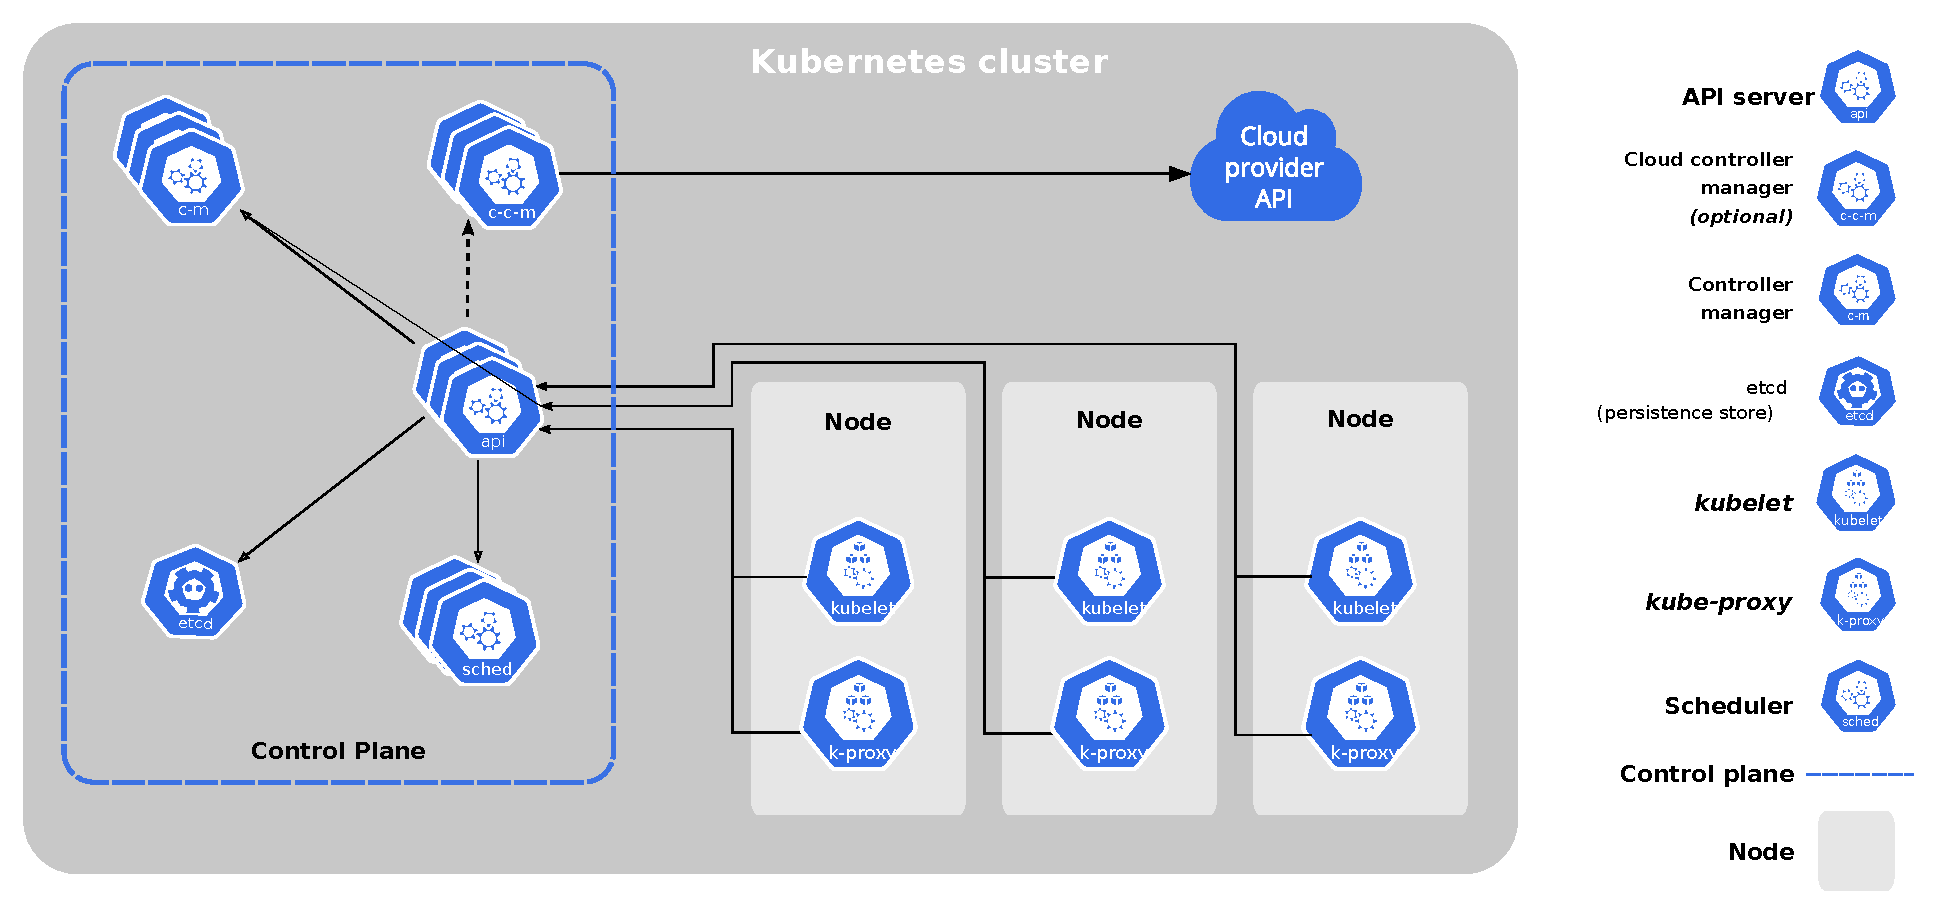
\includegraphics[width=.84\linewidth]{assets/components-of-kubernetes.pdf}
	\legend{Fonte: \citeonline{kubernetesCoreComponentes}}
\end{figure}

\newpage
\subsection{Objetos e serviços Kubernetes}
Além dos componentes do \textit{Control Plane} existem outros objetos e serviços que são fundamentais para a conteinerização, funcionamento do \textit{Kubernetes}, ou são pertinentes a este trabalho. 

\subparagraph{\textit{Pods}:} representa a menor unidade de objeto no \textit{Kubernetes}. Em resumo um \textit{pod} é uma carga de trabalho que é executado em \textit{nodes} do \textit{cluster} no formato de um processo.
\textit{Pod} é considerado um grupo com um ou mais contêineres, os quais compartilham recurso de disco e rede, cada \textit{pod} contém especificação declarativa da execução dos contêineres que possui. A comunicação entre os contêineres de um mesmo \textit{pod} é feita por meio de \textit{inter-process comunication (IPC)}, como semáforos \textit{SystemV}, ou, utilizando a memória compartilhada \textit{POSIX}. Por padrão, contêineres em \textit{pods} distintos não se comunicam por meio de \textit{IPC} sem configuração personalizada. Desse modo, a comunicação entre contêineres em \textit{pods} distintos é concebida via troca de mensagem utilizando protocolo \textit{IP}.
	
\subparagraph{\textit{ReplicaSet}:}
Considerado um serviço responsável pelo controle de réplicas de \textit{pods} solicitado. Assim, o \textit{ReplicaSet} garante a disponibilidade de um número de \textit{pods}.
	
\subparagraph{\textit{Deployments}:}
fornece atualizações declarativas para \textit{pods} e \textit{replicaSets}. Ou seja, o \textit{deployment} é usado para atualização de estado de \textit{pods} e \textit{ReplicaSets}. O uso comum de \textit{deployments} em relação aos \textit{pod} é na atualização de imagem do contêiner, já para \textit{ReplicaSet} seria na atualização no número de réplicas disponíveis desejado.

\subsection{Detalhes de escalonamento}
Para realizar o escalonamento dos \textit{pods}, o \textit{kube-scheduler} executa um fluxo de operações que são separadas em duas categorias: Filtragem e Ranqueamento. Em resumo, a filtragem consiste em investigar \textit{nodes} que são capazes de executar o \textit{pod} a ser escalonado, ou seja, nessa etapa há a seleção dos \textit{nodes} do \textit{cluste} que satisfazem a solicitação de recursos do \textit{pod}. O ranqueamento, por sua vez, classifica os \textit{nodes} eleitos pela filtragem e seleciona o \textit{node} que obter a maior pontuação de acordo a solicitação de recursos do \textit{pod} \cite{Kubescheduler}.

A técnica de escalonamento utilizada pelo \textit{kube-scheduler} é denominada \textit{First-Come-First-Served} (FCFS), conhecido também como \textit{First-In-First-Out} (FIFO), que consiste em escalonar os serviços pela ordem de chegada. Alguns motivos são elencados para defender a escolha dessa técnica, por exemplo, garantia da ausência de inanição e simples implementação algorítmica. Embora exista o consenso que há espaço de melhoria, substituir essa técnica de escalonamento por um algoritmo aprimorado 
requer um estudo de caso específico bem definido \cite{CarastanSantos2019}.

\subsection{Customização do \textit{kube-scheduler}}
\label{customizacao_kube_scheduler}
De acordo com \citeonline{ibm-sched} há 4 meios de customizar o escalonador do \textit{Kubernetes}, que serão abordados nessa seção.

\subparagraph{Alteração do código fonte:}
A primeira técnica consiste em clonar o repositório do código fonte do \textit{Kubernetes}, modificar o comportamento do escalonador padrão, recompilar o projeto e executar o escalonador. Essa prática não é recomendada pois há a necessidade de alinhar o código alterado com o fluxo de execução do \textit{Kubernetes}, o segundo fator que desmotiva esse método, é que o próprio \textit{Kubernetes} oferece meios para alterar o comportamento do escalonador sem a necessidade de alterar o código fonte.

\subparagraph{Múltiplos escalonadores:}
A segunda técnica é executar um escalonador customizado ao lado do escalonador padrão. O escalonador customizado é conteinerizado no formato de \textit{pod} e orquestrado pelo próprio \textit{Kubernetes}. Para que o escalonador padrão e o customizado não disputem os mesmos \textit{pods}, na criação do \textit{pod} é preciso identificar o método de escalonamento por meio do nome do escalonador. Caso contrário, a co-existência de múltiplos escalonadores causa o bloqueio de sincronização. A comunicação do \textit{pod}, abstraído em escalonador de contêineres, com a \textit{API} do \textit{Kubernetes} é custosa. Pois o \textit{pod} irá consumir a \textit{API} do \textit{Kubernetes} por meio do protocolo \ac{HTTP}.

\subparagraph{Extensão do escalonador padrão:}
A terceira solução é denominada Extensão, considerada a solução mais simples, que objetiva adicionar funcionalidades extras ao \textit{kube-scheduler}. Extensão é entendido como a configuração de ganchos (\textit{webhooks}) que o \textit{Kubernetes} oferece para executar filtragem e ranqueamento dos \textit{nodes} de forma customizada. Ganchos devem ser interpretados como gatilhos, que são funções personalizadas que o \textit{Kubernetes} engatilha para alterar algum comportamento padrão ou adicionar novas funcionalidades. Devido a simplicidade, esse método apresenta algumas limitações. A transferência de dados, entre o escalonador customizado e o padrão, é realizada via protocolo \ac{HTTP}, ocasionando custo alto de comunicação. O segundo problema está relacionado com a própria limitação da abordagem, pois altera apenas os procedimentos das fases de filtragem e ranqueamento, não atuando no início nem no fim de nenhuma outra etapa de escalonamento. 

\subparagraph{\textit{Framework} de escalonamento:}
O quarto método de customizar o escalonador padrão do \textit{Kubernetes} é denominado \textit{framework} de escalonamento. Essa técnica consiste em adicionar pontos de extensão no escalonador padrão do \textit{Kubernetes}, chamados \textit{plugins}, que são incluídos em tempo de compilação. Os \textit{plugins} podem ser habilitados, desabilitados e reordenados. \textit{Plugins} são adicionados nos ciclos padrões de escalonamento -- \textit{scheduling} e \textit{binding}. No ciclo \textit{scheduling} está habilitado a extensão por meio de 8 \textit{plugins}: \textit{sort, PreFilter, Filter, PreScore, Score, NormalizeScore, Reserve, Permit}. Já, na fase de \textit{binding} há 3 pontos de extensão: \textit{PreBind, Bind, PostBind}. O presente trabalho não realizará revisão completa sobre os pontos de extensão, uma vez que a documentação explora este assunto de forma ampla \cite{schedulerframework}.

\subsection{Alta disponibilidade}
A configuração de um \textit{cluster} \textit{Kubernetes} visando alta disponibilidade é essencial para o uso de aplicações conteinerizadas em produção. A alta disponibilidade é alcançada a partir da replicação do \textit{node} \textit{master}, com isso, eliminando um único ponto de falha para os componentes do \textit{Control Plane}, que são fundamentais para o funcionamento do \textit{Kubernetes} \cite{Kubeha}.

Em uma implantação do \textit{Kubernetes} com configuração de alta disponibilidade, a instância do banco de dados \textit{etcd} será replicadas utilizando um algoritmo de consenso, e todos os servidores \textit{kube-apiserver} estarão disponíveis por meio de um balanceador de carga. Enquanto que os demais componentes (\textit{Kube-controller-manager}, \textit{Cloud-controller-manager}, \textit{kube-scheduler}) estarão apenas com uma instância ativa no \textit{cluster}. Portanto, a replicação do \textit{node master} torna-se uma solução eficaz para tolerância a falhas, contudo, não resolve a escalabilidade do problema de escalonamento. Isso ocorro porque as réplicas do \textit{kube-scheduler} não atuam em conjunto no processo de escalonamento.

\section{Microsserviços}

De acordo com \citeonline{FowlerMicrosservice} não há definição precisa de microsserviços, contudo, existem algumas características em comum acerca das implantações dessa arquitetura. Como por exemplo, um conjunto de serviços que constitui um sistema, controle descentralizado da informação, automação da implantação de software e uso heterogêneo de linguagens de programação e banco de dados.

\subsection{Definições e conceitos}
A arquitetura de microsserviços visa o desenvolvimento de um sistema como um conjunto de serviços sucintos seccionados em processos independentes, podendo ou não compartilhar o mesmo hospedeiro \cite{lewis2012microservices}. Isto é, microsserviços são pequenas aplicações que podem ser implantadas, escaladas e testadas independentemente, que possuem um conjunto limitado de funcionalidades para resolver um só objetivo. Uma única responsabilidade, por um lado, deve ser interpretado como uma única razão para mudar ou uma única razão para ser substituído. Por outro lado, deve ser interpretada como um sistema que possuí uma funcionalidade apenas, o qual tem de ser facilmente  compreendido fora de seu contexto. Considera-se que o conceito de microsserviço está relacionado com a filosofia \textit{unix}: "Escreva programas que façam apenas uma coisa, mas que façam bem feita" e "Escreva programas que trabalhem juntos" \cite{thones2015microservices}.

Para a interação entre os serviços que compõe um sistema, os microsserviços se beneficiam de protocolos leves para troca de mensagem, como \ac{RPC}, protocolo de mensagens e, se for necessário, é possível utilizar \ac{HTTP}. O \ac{HTTP} é a forma habitual  que o navegador carrega páginas da \ac{WWW}, enquanto que, \ac{RPC} e fila de mensagens são protocolos comumente empregado para comunicação de sistemas distribuídos \cite{ericraymond2003}.

\subsection{Do monolítico ao microsserviços}
Em engenharia de software, um sistema monolítico constituí-se de uma única unidade, todo código é vinculado a um único processo. Aplicações comerciais geralmente são dividas em três partes, lado cliente, habitualmente uma página \textit{web}, banco de dados e uma aplicação do lado servidor. Em uma aplicação \textit{web}, esse servidor lida com o \ac{HTTP}, executa a regra de domínio e persiste informações no banco de dados. O sistema do lado servidor é considerado um monolítico. Por consequência, qualquer alteração no sistema influenciará em construir e implantar uma nova versão da aplicação.

Desenvolver de forma monolítica é a maneira natural de construir sistemas, toda a lógica é gerenciada por um único processo. O projeto para esse tipo de sistema equivale a segregar as partes/módulos do sistema por meio das técnicas de programação da linguagem utilizada, por exemplo classes, interfaces, hierarquia, etc. Entretanto, sistemas monolíticos não performam na questão de escalabilidade. Pois escalar monolítico consiste em replicar o sistema de forma integral. Já em uma aplicação baseada em microsserviços proporciona um escalabilidade inteligente, pois replica as partes de acordo com a necessidade por meio de um balanceador de carga dedicado para cada serviço, como ilustra a figura \ref{monolitico-microsservico}.

\begin{figure}[ht!]
    \caption{\label{monolitico-microsservico}Comparação entre Monolítico e Microsserviços}
    \centering
    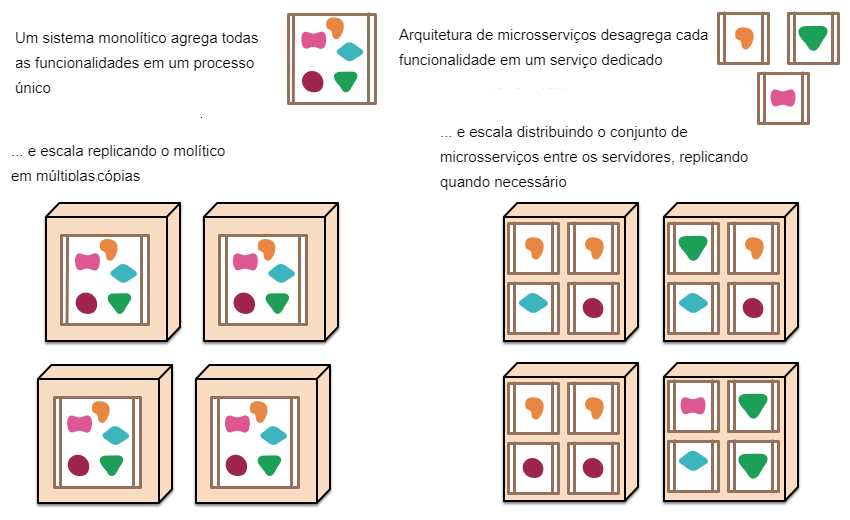
\includegraphics[width=0.85\linewidth]{assets/monilitico-microsservico.png}
    \legend{Fonte: \citeonline{FowlerMicrosservice}}
\end{figure}

\subsection{Projeto de Microsserviço guiado pelo \textit{DDD}}
O \ac{DDD}, no contexto de engenharia de software, é uma metodologia que conecta conceitos de linguagem de programação, por exemplo nome de classes, métodos, e atributos com o domínio do negócio \cite{DDD}. Define-se domínio como a área de conhecimento, ou seja, as funcionalidades do sistema a nível de negócio \cite{evans2014domain}.

De acordo com \citeonline{FowlerMicrosservice}, o \ac{DDD} decompõe um domínio complexo em múltiplas partes, na literatura é definido como contextos delimitados (\textit{bounded context}), como também visa o projeto do relacionamento entre esses. Este padrão é utilizada tanto para projetar sistemas monolíticos quanto distribuída em microsserviços. Nota-se uma correlação semântica entre um serviço e um contexto delimitado, que reforça a separação lógica do domínio em serviços isolados, consequentemente, em microsserviços. Isto é, o contexto delimitado do conceito do \ac{DDD} se torna um excelente candidato à um microsserviço \cite{newman2015building}. Contudo, nem todo contexto delimitado deve ser relacionado à um microsserviço independente. Segundo o criador do \ac{DDD}, Eric Evans, há diferentes tipos de contexto delimitado que não mapeiam diretamente a um serviço isolado.

Um dos desafios de projetar sistemas baseados em serviços distribuídos é determinar a granularidade em termos de escopo e complexidade do microsserviço. O conjunto de funções que definem o microsserviço não deve ser extremamente simplista, muito menos agregar muita complexidade \cite{merson2020modeling}. Portanto, para permitir o gerenciamento descentralizado de acordo com o contexto do domínio, o ideal é unir os princípios do \ac{DDD} com a arquitetura de microsserviços.

\section{Escalonamento de Tarefas}

Escalonamento consiste um processo de tomada de decisão, que é usado regularmente no ramo da manufatura, serviços industriais e sistemas operacionais. O escalonamento lida com alocação de recursos para tarefas em determinados períodos de tempo, visando otimizar um ou mais objetivos \cite{pinedo2012scheduling}. Sendo alguns desses objetivos, por exemplo, redução do tempo de espera das tarefas, maximização do uso de recursos (espalhamento), ou minimização do uso total de recursos (agrupamento).

Neste trabalho, escalonamento é um procedimento o qual soluciona alocações de recursos computacionais. Recursos refletem em quantidade mensurável de memória, processamento e dispositivos de rede de um, ou conjunto, de nós computacionais  (também denominado por máquinas). Segundo \citeonline{brucker1999resource}, considere que $m$ máquinas $M_j (j = 1, \dots, m)$ deverão processar $n$ trabalhos $J_i (i = 1, \dots, n)$. Vinculado a cada trabalho $J_i$ há um número $n_i$ de tarefas $(O_{i1}, O_{i2}, \dots, O_{in_i})$, para cada tarefa há uma solicitação de recursos $p_{ij}$. Dessa forma, o escalonamento é um processo de tomada de decisão que, a partir da requisição de recursos da tarefa,  investigará os nós computacionais  factíveis e indicará o escalonamento ideal de $J_i$ para $M_j$ de acordo com a otimização de alguma métrica de interesse. Um escalonamento válido para alocação de trabalhos pode ser representado por meio do diagrama de Gantt, como exemplifica a figura \ref{gantt-schedulling}.

\begin{figure}[ht!]
    \caption{\label{gantt-schedulling}Visualização escalonamento por meio do diagrama de Gantt}
    \centering
    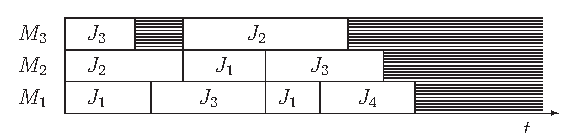
\includegraphics[width=\linewidth]{assets/gantt-scheduling.pdf}
    \legend{Fonte: \citeonline{brucker1999resource}}
\end{figure}

De acordo com \cite{pinedo2012scheduling}, o problema de escalonamento é representado por uma tripla $\alpha|\beta|\gamma$. O campo $\alpha$ representa o ambiente, interpreta-se como o perfil da arquitetura que detém os recursos em que os trabalhos serão escalonados. O campo $\beta$ define detalhes de processamento e restrições que estão vinculados ao trabalho, pode conter nenhuma, uma única ou várias entradas. Já o campo $\gamma$ descreve a função objetivo a qual visa otimização de alguma métrica de interesse, normalmente contém apenas uma entrada.

Para este trabalho, a entrada $\gamma$ será definida pelo perfil \textbf{Máquinas em Paralelo com Diferentes Velocidades} e é representado pelo rótulo $Qm$. Este cenário consiste em $m$ máquinas heterogêneas, que não necessariamente possuem a mesma quantidade de recursos. Considera-se a principal abordagem das nuvens computacionais atualmente \cite{krauter2002taxonomy}.

A entrada $\beta$ é definida pelo conjunto \textbf{Prazo ou \textit{deadline}} ($P$), \textbf{Restrição de Elegibilidade} ($M$) e \textbf{Processamento em Lote} ($batch(b)$). Se o rótulo $P$ está presente em $\beta$, então para cada trabalho $J_{k}$ será atribuído um prazo de entrega $P_{k}$, dessa forma, $J_k$ não deve ser escalonado após o prazo $P_{k}$. Se $P$ não está incluído em $\beta$, logo não há restrição de \textit{deadline} de escalonamento. O rótulo $M$ denota que nem todas as máquinas são capazes de processar o trabalho $J_{k}$, assim, o conjunto $M_{k}$ representa as máquinas que satisfazem as restrições de $J_{k}$, que por consequência, são elegíveis ao escalonamento. Por último, se há rótulo $batch(b)$ em $\beta$, então, uma máquina é apta a processar quantidade $b$ de trabalhos de forma simultânea.

Portanto, $\beta=\{P, M, batch(b)\}$. O campo $\gamma$, que está relacionado com métricas de escalonamento e funções objetivos, será desenvolvido na seção subsequente.

\subsection{Métricas de Escalonamento e Função Objetivo}
De acordo com \cite{Feitelson98}, há um conjunto de métricas relevantes a respeito do desempenho de algoritmos de escalonamentos. O presente trabalho visa a otimização das seguintes métricas: tempo de espera de escalonamento, \textit{makespan}. Além disso, análise do comportamento do \textit{slowdown}.

\subsubsection{Tempo de Espera}
Considere $Submetido_k$ o momento em que o trabalho $J_k$ foi submetido à plataforma, $Inicio_k$ o momento em que o trabalho $J_k$ iniciou sua execução. A Equação \ref{eq:1} mensura o tempo de espera, ou seja, o tempo que o trabalho permanece na fila até ser escalonado. Para um trabalho $J_k$ o tempo de espera $T_k$ é determinado pela equação:

\begin{equation} \label{eq:1}
T_k = Inicio_k - Submetido_k
\end{equation}

Minimização do tempo de espera é um problema de escalonamento conhecido importante no fornecimento de \textit{Quality of Service (QoS)} em muitas indústrias \cite{Ye2007}. Por ser classificado como um problema \textit{NP-Hard} \cite{Kubiak1993}, na literatura é encontrada diferentes heurísticas que aproximam-se da solução ideal, pois não há algoritmo de busca eficiente que encontre uma sequência ótima \cite{Ye2007}.

\subsubsection{\textit{Makespan}}
A próxima métrica a ser considerada é o \textit{makespan}, que é uma métrica diretamente vinculada ao tempo de completude de um trabalho. O cálculo é definido pelo tempo de término da última tarefa de um trabalho a deixar o sistema. Considere que um trabalho $J_k$ possui $n$ tarefas vinculadas $O_{k,1}, O_{k,2}, ..., O_{k,n}$, e para cada tarefa $O_{k,i}$ há vinculado tempo de finalização $C_i$, assim o \textit{makespan} $C_{max, k}$ de $J_k$ é calculado de acordo com a equação:

\begin{equation}
C_{max,k} = max(C_1, C_2, ..., C_n) 
\end{equation}

A minimização do \textit{makespan} resulta na otimização da utilização dos recursos computacionais \cite{pinedo2012scheduling}. Pois o \textit{makespan} está relacionado ao tempo que o trabalho permanece na plataforma, a sua minimização acarreta em melhor agrupamento do escalonamento, que por consequência, ocorrendo a liberação do uso de recursos em um menor período de tempo.

\subsubsection{\textit{Slowdown}}
Por último, outra métrica abordada neste trabalho é o \textit{slowdown}, que é definido pela relação entre o tempo total que o trabalho permaneceu na plataforma com o tempo atual de processamento gasto com o mesmo. Assim o \textit{slowdown} $Sd_k$ de $J_k$  é definido pela Equação \ref{eq:2}:

\begin{equation} \label{eq:2}
Sd_{k} = \frac{T_{k} + P_{k}}{P_{k}}
\end{equation}

\(P_{k}\) é o tempo de processamento de \(J_k\). O propósito do \textit{slowdown} é estabelecer  proporção entre tempo de espera de um trabalho em relação ao seu tempo de processamento \cite{Maccio2018}, com o objetivo de atribuir uma distribuição equilibrada do tempo de espera entre os trabalhos com diferentes cargas de trabalho \cite{CarastanSantos2019}.

\subsubsection{Função Objetivo}
Portanto o campo $\gamma$ (função objetivo) da definição de escalonamento refere-se à minimização do tempo de espera, \textit{makespan}, logo, $\gamma = T, C_{max}$. Em cenários como \ac{HPC}, os resultados visados por meio da otimização desse conjunto de métricas são: Melhor \textit{QoS} por meio da minimização do tempo de espera; Otimizar a utilização dos recursos computacionais mediante a minimização do \textit{makespan}; Analisar o comportamento do \textit{slowdown}.

\subsection{Escalonamento Distribuído}

Aplicações atuais fundamentam-se na análise e processamento de um grande volume de dados, como por exemplo, \textit{Data Mining}, \textit{Machine Learning}, \textit{Deep Learning} e banco de dados. Dessa forma, conforme a demanda de poder computacional cresce, as estruturas responsáveis pela execução dessas aplicações os acompanham, refletindo no aumento de complexidade tanto em tamanho como em algoritmos refinados de gerenciamento \cite{Wang2016LoadbalancedAL}. A nível de comparação desse reflexo, a empresa \textit{Google} executa centenas de milhares de cargas de trabalho, de muitos milhares de aplicativos em uma conjunto de \textit{clusters}, cada qual com até dezenas de milhares de máquinas \cite{Google2015Borg}. Por consequência, os componentes internos de gerenciamento de um \textit{data center} de larga escala deve resolver os problemas internos com algoritmos complexos e sofisticados para cada tipo de cenário.

O escalonamento é um tema amplamente pesquisado, desde de otimização por meio de processamento em \textit{GPU} \cite{Nesi2018ScheduleGPU} como também baseado em arquitetura descentralizada empregando conceitos de \textit{blockchain} \cite{loch2021novel}. De acordo com a literatura, escalonamento distribuído, hoje, é requisito fundamental para \textit{Data Centers} de larga escala \cite{Google2015Borg, Wang2019Pigeon}. Uma vez que, a principal dificuldade da abordagem centralizada está na escalabilidade e nos métodos de tolerâncias a falhas, que degradam por completo as métricas de \ac{QOS}. O escalonamento, no formato distribuído, resolve este problema de forma elaborada removendo o único ponto de falha ao particionar as requisições de alocação de recursos em um sistema distribuído.

\section{Trabalhos Relacionados}

A área de escalonamento de tarefas é estudada a décadas, considera-se um ramo com intersecção em diferentes campos da ciência da computação. Um dos principais fatores que impulsionam a intersecção entre as áreas está na natureza do problema de escalonamento, pois na maioria dos casos resolver um problema de escalonamento reflete em otimizar um problema \textit{NP-difícil}. Dessa forma, na literatura, encontra-se diferentes pesquisas que refletem em soluções heurísticas e refinadas, muitas vezes relacionadas com a área de inteligência artificial. Por se tratar da solução de um problema \textit{np-difícil}, a solução computada basta ser boa o suficiente para um cenário específico, sendo assim, a solução encontrada nem sempre é refletida na ótima global.

Esta seção analisará trabalhos recentes da literatura que possuem relação com escalonamento de contêineres. Por ainda se tratar de um recorte amplo na área de escalonamento, aqui analisou-se diferentes trabalhos que atacam diferentes características, seja relacionado com otimização energética em \textit{data centers} como também trabalhos que buscaram otimizar o desempenho de escalonamento.

\subsection{Redução do custo energético}
No trabalho de \citeonline{sureshkumar2017optimizing} os autores propuseram um algoritmo de escalonamento de contêineres, para a tecnologia \textit{docker}, baseado em balanceamento de carga. O algoritmo consiste em um limiar calculado a partir da sobrecarga do \textit{cluster}, o objetivo do limiar é que as cargas dos contêineres não sejam muito altas e baixas. Quando a carga ultrapassa o limiar, um novo contêiner é criado no balanceamento de carga. Por outro lado, quando a carga é muito baixa, o contêiner é destruído com o objetivo de economizar custo energético.

\subsection{Otimização multi objetivo}
Em \citeonline{liu2018new} os autores desenvolveram um novo algoritmo de escalonamento de contêineres denominado \textit{multipot}. Neste projeto foi estudado múltiplos critérios para a seleção de um \textit{node} para provisionar o contêiner. O algoritmo considera cinco métricas chaves:
\begin{enumerate}
	\item Uso de CPU de cada \textit{node};
	\item Uso de memória de cada \textit{node};
	\item Tempo da transmissão da imagem do contêiner na internet;
	\item Associação entre os contêineres e os \textit{nodes};
	\item Agrupamento de contêineres.
\end{enumerate}
Todas essas métricas foram consideradas, pois, de acordo com os autores, afetam no desempenho das aplicações que estão sendo executadas pelos contêineres. A função objetivo de escalonamento é a otimização da composição de todas as métricas chaves, ou seja, para cada métrica chave é relacionado um escore, esses escores são agrupados em uma função de composição que representa a função objetivo.

Em \citeonline{menouer2019new} foi desenvolvido uma nova estratégia de escalonamento baseado em um algoritmo de decisão multi-critério. A abordagem consiste em escalonar contêineres baseado em três critérios que estão relacionados a todos os \textit{nodes}  que constitui a infraestrutura de nuvem: (1) O número de contêineres em execução; (2) A disponibilidade de CPU; (3) A disponibilidade do espaço de memória.

Em \citeonline{menouer2019power} os autores utilizaram técnicas refinadas de \textit{machine learning} em um ambiente de nuvem para construção de um escalonador de contêineres. O objetivo dessa abordagem é reduzir o consumo energético de infraestruturas de nuvens heterogêneas. O principio corresponde a dois passos denominados (1) aprender e (2) escalonar, que são aplicados a cada novo contêiner que é submetido à plataforma. No passo (1) é estimado o consumo energético de cada \textit{node}, logo, é elencado grupos de \textit{nodes} que formam uma estrutura de nuvem heterogênea em um \textit{cluster} de acordo com o seu consumo energético.
Já no passo (2), é selecionado o \textit{node} que corresponde  ao menor consumo energético. O algoritmo foi implementado para a plataforma \textit{docker swarm}.

\subsection{Considerações parciais}
Está seção elencou alguns do trabalhos encontrados na literatura acerca do tema escalonamento de contêineres. Nota-se que os trabalhos envolvidos possuem definição de parâmetros e métricas de otimização, como por exemplo: consumo energético, desempenho. Por se tratar de um recorte grande na literatura, o tema escalonamento abre espaço para implementação de diferentes soluções para o problema. Todavia, os trabalhos relacionados aqui elencados não consideram o fator escalabilidade, não há nenhuma solução distribuída. A escassez de projetos de escalonamento de contêineres que envolvam o desenvolvimento de uma arquitetura distribuída, é uma das principais motivações para o presente trabalho.

% ----------------------------------------------------------

% ----------------------------------------------------------
% Trabalhos relacionados
% ----------------------------------------------------------
% \chapter{Trabalhos Relacionados}
%%
%%\textcolor{red}{Linha escalonadores distribuidos: revisao do Wilton}
%%
%%MapReduce, Spark, XYZ
%%Conclusão: a minha ideia é que pode ser usado qualquer escalonador, desde que seja possível representar como microsserviço (stateless).
%%
%%\textcolor{red}{Tecer comentários sobre TF: replicas ja foram usadas para contornar falhas. %%\url{https://gkoslovski.github.io/files/ijguc-2019.pdf}}
%%
%%Tabela de conclusao. Colunas: 1 ref, 2 foco, 3 container/VM/tarefa. Mostrar que microsservico é uma opção viavel.
%%
%%A área de escalonamento possui diversas referencias fortes em diversas áreas. Entretanto, a conteinerização é um termo recente comparado a toda história 

A área de escalonamento de tarefas é estudada a décadas, considera-se um ramo com intersecção em diferentes campos da ciência da computação. Um dos principais fatores que impulsionam a intersecção entre as áreas está na natureza do problema de escalonamento, pois na maioria dos casos resolver um problema de escalonamento reflete em otimizar um problema \textit{NP-difícil}. Dessa forma, na literatura, encontra-se diferentes pesquisas que refletem em soluções heurísticas e refinadas, muitas vezes relacionadas com a área de inteligência artificial. Por se tratar da solução de um problema \textit{np-difícil}, a solução computada basta ser boa o suficiente para um cenário específico, sendo assim, a solução encontrada nem sempre é refletida na ótima global.

Esta seção analisará trabalhos recentes da literatura que possuem relação com escalonamento de contêineres. Por ainda se tratar de um recorte amplo na área de escalonamento, aqui analisou-se diferentes trabalhos que atacam diferentes características, seja relacionado com otimização energética em \textit{data centers} como também trabalhos que buscaram otimizar o desempenho de escalonamento.

\section{Redução do custo energético}
No trabalho de \citeonline{sureshkumar2017optimizing} os autores propuseram um algoritmo de escalonamento de contêineres, para a tecnologia \textit{docker}, baseado em balanceamento de carga. O algoritmo consiste em um limiar calculado a partir da sobrecarga do \textit{cluster}, o objetivo do limiar é que as cargas dos contêineres não sejam muito altas e baixas. Quando a carga ultrapassa o limiar, um novo contêiner é criado no balanceamento de carga. Por outro lado, quando a carga é muito baixa, o contêiner é destruído com o objetivo de economizar custo energético.

\section{Otimização multi objetivo}
Em \citeonline{liu2018new} os autores desenvolveram um novo algoritmo de escalonamento de contêineres denominado \textit{multipot}. Neste projeto foi estudado múltiplos critérios para a seleção de um \textit{node} para provisionar o contêiner. O algoritmo considera cinco métricas chaves:
\begin{enumerate}
	\item Uso de CPU de cada \textit{node};
	\item Uso de memória de cada \textit{node};
	\item Tempo da transmissão da imagem do contêiner na internet;
	\item Associação entre os contêineres e os \textit{nodes};
	\item Agrupamento de contêineres.
\end{enumerate}
Todas essas métricas foram consideradas, pois, de acordo com os autores, afetam no desempenho das aplicações que estão sendo executadas pelos contêineres. A função objetivo de escalonamento é a otimização da composição de todas as métricas chaves, ou seja, para cada métrica chave é relacionado um escore, esses escores são agrupados em uma função de composição que representa a função objetivo.

Em \citeonline{menouer2019new} foi desenvolvido uma nova estratégia de escalonamento baseado em um algoritmo de decisão multi-critério. A abordagem consiste em escalonar contêineres baseado em três critérios que estão relacionados a todos os \textit{nodes}  que constitui a infraestrutura de nuvem: (1) O número de contêineres em execução; (2) A disponibilidade de CPU; (3) A disponibilidade do espaço de memória.

Em \citeonline{menouer2019power} os autores utilizaram técnicas refinadas de \textit{machine learning} em um ambiente de nuvem para construção de um escalonador de contêineres. O objetivo dessa abordagem é reduzir o consumo energético de infraestruturas de nuvens heterogêneas. O principio corresponde a dois passos denominados (1) aprender e (2) escalonar, que são aplicados a cada novo contêiner que é submetido à plataforma. No passo (1) é estimado o consumo energético de cada \textit{node}, logo, é elencado grupos de \textit{nodes} que formam uma estrutura de nuvem heterogênea em um \textit{cluster} de acordo com o seu consumo energético.
Já no passo (2), é selecionado o \textit{node} que corresponde  ao menor consumo energético. O algoritmo foi implementado para a plataforma \textit{docker swarm}.

\section{Considerações parciais}
Está seção elencou alguns do trabalhos encontrados na literatura acerca do tema escalonamento de contêineres. Nota-se que os trabalhos envolvidos possuem definição de parâmetros e métricas de otimização, como por exemplo: consumo energético, desempenho. Por se tratar de um recorte grande na literatura, o tema escalonamento abre espaço para implementação de diferentes soluções para o problema. Todavia, os trabalhos relacionados aqui elencados não consideram o fator escalabilidade, não há nenhuma solução distribuída. A escassez de projetos de escalonamento de contêineres que envolvam o desenvolvimento de uma arquitetura distribuída, é uma das principais motivações para o presente trabalho.
 


% ----------------------------------------------------------

% ----------------------------------------------------------
% Proposta
% ----------------------------------------------------------
\chapter{KMS - \textit{Kubernetes Micro Scheduler}\label{cap-proposta}}

Este capítulo tem como objetivo apresentar os processos de desenvolvimento do escalonador distribuído proposto, denominado \ac{KMS}. A escolha do nome está concentrada na etimologia da palavra \textbf{micro}, a qual significa \textbf{pequeno}, visto que um dos principais objetivos do presente trabalho é distribuir o escalonador utilizando conceitos de \textbf{micro}sserviços. Ou seja, fragmentar um escalonador monolítico em pequenos sistemas que operam de forma independentes, mas em conjunto refletem um sistema distribuído robusto.

No início do capítulo é apresentado um comparativo entre o \ac{KMS} com as atuais abordagens de escalonamento do \textit{Kubernetes}, o principal objetivo nesta seção é confrontar as arquiteturas em cenários de falhas. Ao passo que, as seções subsequentes são dedicadas ao funcionamento dos componentes do \ac{KMS}, como também as trocas de mensagens. Exceto a Seção 3.2, que é destinada à apresentar a documentação baseada na engenharia de requisitos para delimitar o escopo do projeto.

%O presente trabalho visa o desenvolvimento de um escalonador distribuído, baseado em microsserviços, e a sua implantação no \textit{Kubernetes}. Dessa forma, os principais objetivos do escalonador proposto são ampliar a escalabilidade visando otimizar as métricas de tempo de espera de escalonamento e \textit{makespan}, como também tratar as falhas de forma competente.

%O desafio inicial é a identificação dos microsserviços a partir de uma abordagem fundamentada em sistemas distribuídos. O segundo desafio é relacionado ao desenvolvimento do projeto, o qual será visado um sistema documentado, consistente e tolerante a falhas, alcançados por meio de uma arquitetura robusta e replicável. O terceiro desafio compreende na implantação da solução para o \textit{Kubernetes}, como também os resultados a partir das métricas de interesse.

\section{Comparativo com abordagem padrão do \textit{Kubernetes}}
A visualização da proposta e do desempenho esperado do escalonador proposto é notável ao ser comparado com as demais abordagens de escalonamento que o \textit{Kubernetes} oferece (com e sem réplica do \textit{node master)}, como esboça a Figura \ref{fig:comp_sched}.

A figura representa o comportamento de três métodos de escalonamento de contêineres: Escalonador padrão \textit{Kubernetes} com \textit{(1)} e sem \textit{(2)} réplica e o escalonador distribuído proposto \textit{(3)} em um período de tempo dividido em eventos de escalonamento. No primeiro evento de escalonamento há uma solicitação de 100\% de uso dos recursos, e em todas as abordagens o escalonamento é executado com sucesso, pois os recursos estavam disponíveis e não ocorreram falhas. No segundo evento há uma nova solicitação que consome 50\% dos recursos, entretanto, houve a simulação de uma falha do tipo \textit{crash}. Por conta disso, a abordagem \textit{(1)} utilizará um evento de escalonamento para reinicialização do sistema e a abordagem \textit{(2)} redirecionará as requisições para a réplica de escalonamento. Diferente disso, o escalonador distribuído \textit{(3)} é capaz de executar o escalonamento parcial, dado que a falha ocorreu em apenas uma unidade do sistema distribuído. A principal consequência no comportamento do escalonador \textit{(1)} e \textit{(2)} é no atraso das requisições em efeito cascata. Por consequência, todas as requisições que excedem a capacidade de recursos são atrasadas para o próximo passo de escalonamento, causando degradamento do tempo de espera e \textit{slowdown}.

\begin{figure}[h!]
	\caption{\label{fig:comp_sched}Comparação das abordagens de escalonamento}
	\centering
	% \includegraphics[width=\linewidth]{figuras/schedule-proposal.png}
	% \hspace*{-.85in}
	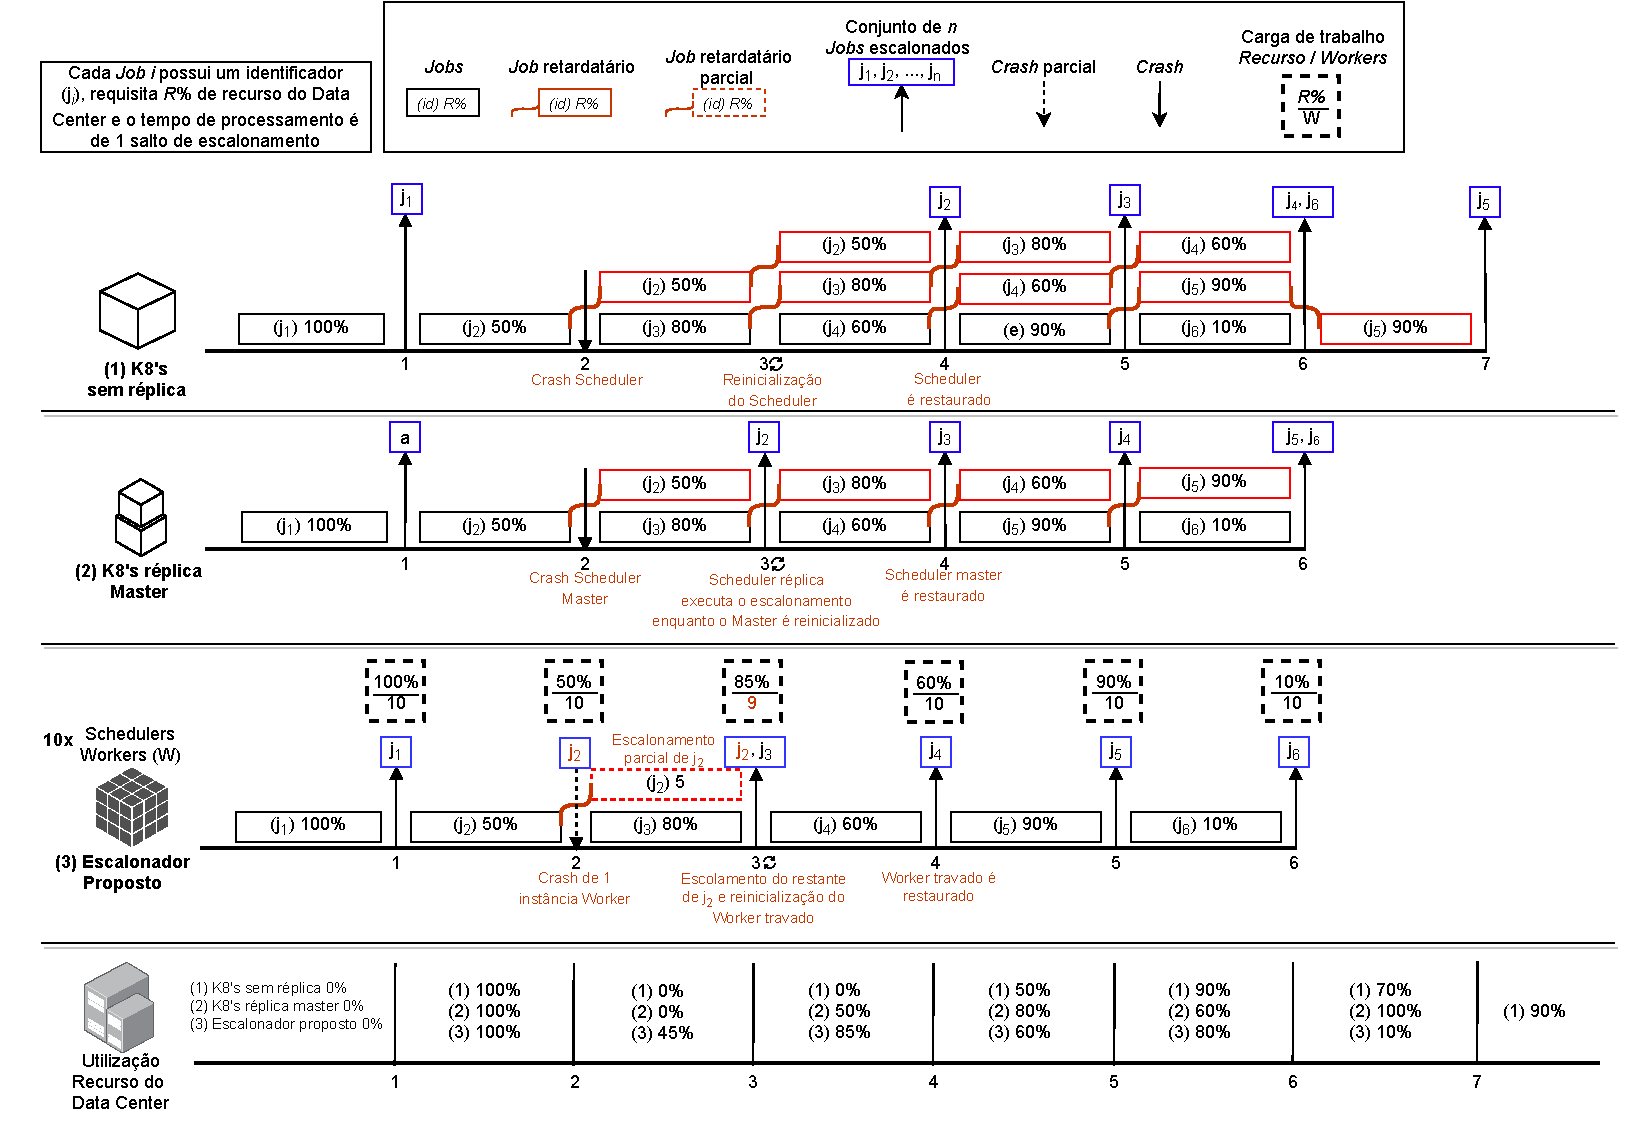
\includegraphics[width=1\linewidth]{assets/schedule-proposal.drawio.pdf}
	\legend{Fonte: O autor}
\end{figure}



\section{Levantamento de Requisitos}

Nessa seção objetiva-se desenvolver uma documentação compreensível do sistema distribuído proposto guiado pela engenharia de requisitos. O levantamento de requisitos é o passo inicial para entendimento do escopo e objetivos do \ac{KMS}, foi desenvolvido utilizando a técnica de análise de cenário e objetivos desejados. No contexto do presente trabalho, buscou-se elencar os requisitos funcionais a partir do comportamento do sistema distribuído e suas funcionalidades, já os requisitos não funcionais aqueles que representam as propriedades e restrições desejadas. 

\subparagraph{Requisitos funcionais}
\begin{enumerate}
	\item Escalonar cargas de trabalho utilizando arquitetura hierárquica de sistemas distribuídos, denominada \textit{master/worker};
	\item Particionar o \textit{cluster}. Cada partição será gerenciado por um escalonador dedicado denominado \textit{worker};
	\item \textit{Workers} serão responsáveis por escalonar cargas de trabalhos nos segmentos do \textit{cluster};
	\item Implementação de estratégias de escalonamento conhecidas na literatura, como por exemplo: \textit{Round-Robin}, \textit{Binpack} e \textit{Easy Backfiling}; e
	\item Possibilidade de intercambiar o algoritmo de escalonamento.
\end{enumerate}

\subparagraph{Requisitos não funcionais}
\begin{enumerate}
	\item O escalonador deverá ser compatível com o \textit{Kubernetes};
	\item Executar os microsserviços virtualizados em contêineres;
	\item O sistema não deve conter único ponto de falha, todos os componentes deverão ser distribuídos;
	\item Desenvolver os principais componentes (\textit{Master} e \textit{Worker}) no formato de microsserviços \textit{stateless}.
	\item Desenvolver um sistema distribuído de forma transparente, ou seja, promover acesso aos recursos distribuídos de forma oculta, como se fosse um único sistema para o usuário; e
	\item Utilizar a estratégia de múltiplos escalonadores, como discutido na seção 2.2.4.
\end{enumerate}

\section{Identificação dos Componentes}

Em síntese, o \ac{KMS} consiste em um modelo hierárquico de sistema distribuído, possuindo 2 componentes principais: \textit{Master} e \textit{Worker}. O componente \textit{Master} corresponde ao único ponto de centralização, isso não significa que haverá um único ponto de falha no sistema, mas sim que este componente manterá apenas uma instância ativa executando o trabalho dentre todas as suas réplicas. Ao fazer uma analogia com a arquitetura Produtor/Consumidor, o componente \textit{Worker} corresponde ao Consumidor, pois é responsável por executar as ações de escalonamento do \ac{KMS}, enquanto que o \textit{Master} é interpretado como Produtor, em razão de lidar com a delegação de trabalho.


% Baseado em um modelo hierárquico, o sistema distribuído proposto consiste em dois componentes principais: \textit{master} e \textit{worker}. O componente \textit{master} corresponde ao único ponto de centralização, já o \textit{worker} é \textit{stateless} e replicável. Cada componente possui uma responsabilidade distinta e específica e em conjunto eles representam o \ac{KMS}.

\subsection{\textit{Master}}

O Master é responsável por buscar cargas de trabalho (\textit{pods}) na fila de escalonamento do \textit{Kubernetes}, em seguida distribuir as cargas para os \textit{Workers}.  Ou seja, é um componente relacionado com a delegação de trabalho, considerado o produtor em um sistema distribuído. Um dos princípios do desenvolvimento, não só do componente \textit{Master}, mas de todo o sistema, é implementar uma arquitetura modular a qual seja possível intercambiar entre as técnicas de escalonamento (seguindo os princípios DDD previamente descritos). O primeiro ponto de escalonamento é encontrado na distribuição das cargas de trabalho do \textit{Master} para os \textit{Workers}. Por exemplo, duas estratégias são observadas na Figura \ref{fig:distribuicao_cargas}: \textit{Binpack} e \textit{Spread}. \textit{Binpack} está relacionado com a minimização dos recursos, ou seja, o algoritmo selecionará o mesmo \textit{Worker} enquanto existirem recursos nessa unidade computacional - na imagem o \textit{worker$_1$} está apenas com 40\% de utilização, por isso todos os \textit{pods} estão sendo direcionados a ele. Já o \textit{Spread} possui como objetivo otimizar o balanceamento de carga dos recursos, comumente utilizado \textit{round-robin}, sendo possível notar que as cargas estão sendo distribuídas de forma igualitária entre os \textit{workers}.

\begin{figure}[h!]
	\caption{\label{fig:distribuicao_cargas} Estratégias de distribuição de cargas entre \textit{master} e \textit{workers}}
	\centering
	% \includegraphics[width=\linewidth]{figuras/schedule-proposal.png}
		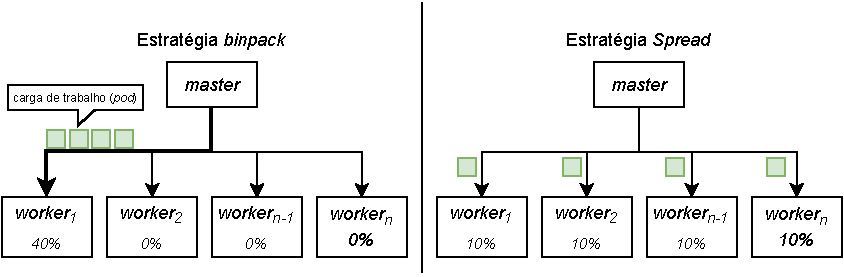
\includegraphics[width=\linewidth]{assets/distribuicao-trabalho.pdf}
	\legend{Fonte: O autor}
\end{figure}

\subsection{\textit{Worker}}

O \textit{Worker} tem como objetivo resolver o escalonamento, ou seja, encontrar um \textit{node} específico para executar o \textit{pod}. A principal característica é ser um componente \textit{stateless} - não armazena estado. Isso é possível, uma vez que foi desenvolvido no formato de microsserviço: recebe uma entrada, executa regras no escopo fechado da entrada e gera uma saída. Dessa forma, a entrada do \textit{Worker} consiste no estado atual do \textit{Cluster} e na lista de \textit{Pods}, que são informados, respectivamente, pela \textit{API} do \textit{Kubernetes} e pelo componente \textit{Master} do \ac{KMS}. Após ler a entrada são executadas operações em relação ao escalonamento, por fim, a saída representa o resultado do escalonamento.

\begin{figure}[h!]
	\caption{\label{fig:microsservico-worker} Comparativo Microsserviço x \textit{Worker}}
	\centering
	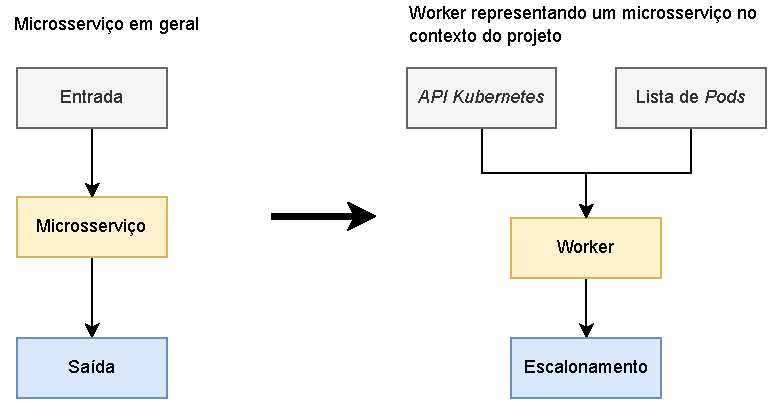
\includegraphics[width=\linewidth]{assets/microsservico-worker.pdf}
	\legend{Fonte: O autor}
\end{figure}

A Figura \ref{fig:microsservico-worker} esboça o comparativo entre entre arquitetura de microsserviço genérica com o componente \textit{Worker}. No \ac{KMS}, o \textit{Worker} é um componente com réplicas, e todas ativas. A ideia é que cada instância gerencie uma partição do \textit{cluster} \textit{Kubernetes}. Por exemplo, considere um \textit{cluster} com \textit{m} nós computacionais e \textit{w} \textit{Workers}, nesse contexto, cada instância do \textit{Worker} será responsável por $m/w$ nós do \textit{cluster}. Isto é, a instância executará o escalonamento no conjunto de nós que pertencem a sua partição.

Ao executar o \ac{KMS} em um \textit{cluster} com 6 nós computacionais e 2 instâncias do componente \textit{Worker}, o \textit{cluster} será seccionado em 2 conjuntos de nós de tamanho 3 (\textit{Tamanho Cluster} / \textit{quantidade réplicas Worker}). Logo, cada instância do \textit{Worker} será responsável por processar o escalonamento da sua respectiva partição, como demonstra a Figura \ref{fig:particionamento-worker}.
Especificamente, tanto o \textit{Worker$_0$} quanto o \textit{Worker$_1$} residem em \textit{Node$_0$}, o que deve-se ao fato que ambas as instâncias foram escalonadas pelo escalonador padrão do \textit{Kubernetes}, que tomou a decisão, neste exemplo de forma hipotética, de escalonar as duas réplicas no mesmo nó computacional. Os componentes internos do \ac{KMS} são escalonados pelo escalonador padrão do \textit{Kubernetes}.

\begin{figure}[h!]
	\caption{\label{fig:particionamento-worker} Particionamento do \textit{cluster} entre \textit{workers}}
	\centering
	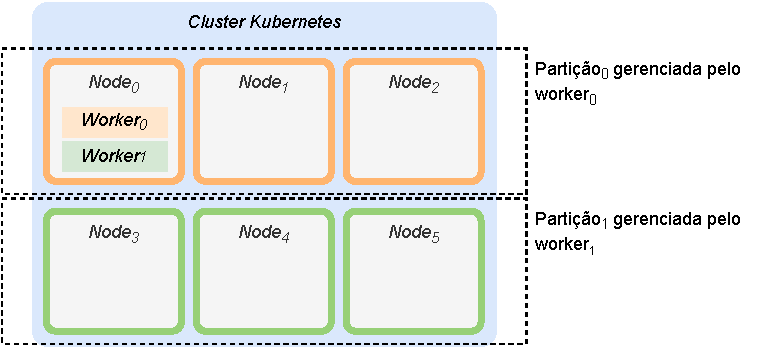
\includegraphics[width=\linewidth]{assets/particionamento-worker.pdf}
	\legend{Fonte: O autor}
\end{figure}

\subsection{Relação \textit{Master}-\textit{Worker}}
As subseções anteriores 3.3.1 e 3.3.2 se encarregaram de apresentar os componentes de forma isolada, nesta subseção objetiva-se sintetizar o funcionamento do \ac{KMS} como um todo. Aqui o principal objetivo é relacionar os componentes \textit{Master} e \textit{Worker}. Em resumo, o \ac{KMS} consiste em 3 passos objetivos: (1) Buscar os \textit{Pods} na fila de escalonamento interna do \textit{Kubernetes}, (2) Distribuir as cargas de trabalho entre os \textit{Workers} e (3) Executar o escalonamento.

%no formato de microsserviço, a ideia é que cada unidade execute o escalonamento em uma partição específica do \textit{cluster}. Dessa forma, ao se executar \textit{n} \textit{workers} então o \textit{cluster} será particionado em \textit{n} partes, como esboça a Figura \ref{fig:worker}.

%\begin{figure}[h!]
%	\caption{\label{fig:worker} particionamento do \textit{cluster} entre \textit{workers}}
%	\centering
%	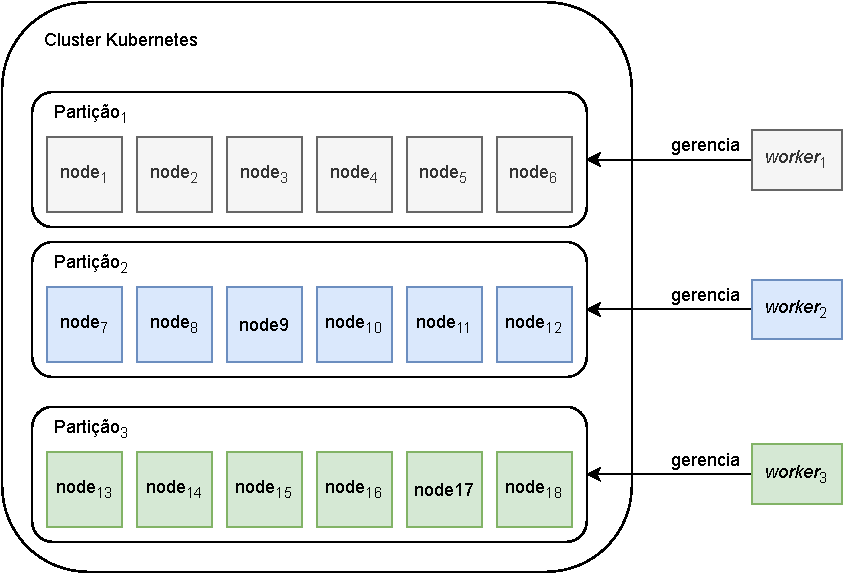
\includegraphics[width=.80\linewidth]{assets/worker.pdf}
%	\legend{Fonte: O autor}
%\end{figure}

%A comunicação entre o sistema distribuído proposto e o \textit{Kubernetes} é efetuada pelo protocolo \ac{HTTP}, em resumo, o \textit{Kubernetes} expõe um servidor \textit{Web} que pode ser consumido por qualquer componente interno. No contexto do presente trabalho, o \textit{Master} consumirá a \textit{API} para buscar os contêineres que estão na fila de escalonamento. Na mesma linha de pensamento, o componente \textit{Worker} se comunicará com a \textit{API} para enviar ordens de escalonamento. Por outro lado, a comunicação entre o componente \textit{master} e \textit{worker} será efetivada via protocolo \textit{gRPC}. Protocolo de comunicação projetado pela \textit{Google}, a principal característica é a performance de alta velocidade entre \textit{microsserviços}.
%O fluxo de execução do sistema distribuído proposto é representado pelo diagrama de fluxo esboçado pela Figura \ref{fig:flow_diagram}.

\begin{figure}[h!]
	\caption{\label{fig:relacao-master-worker}Diagrama de Fluxo}
	\centering
	% \includegraphics[width=0.3\linewidth]{figuras/schedule-proposal.png}
	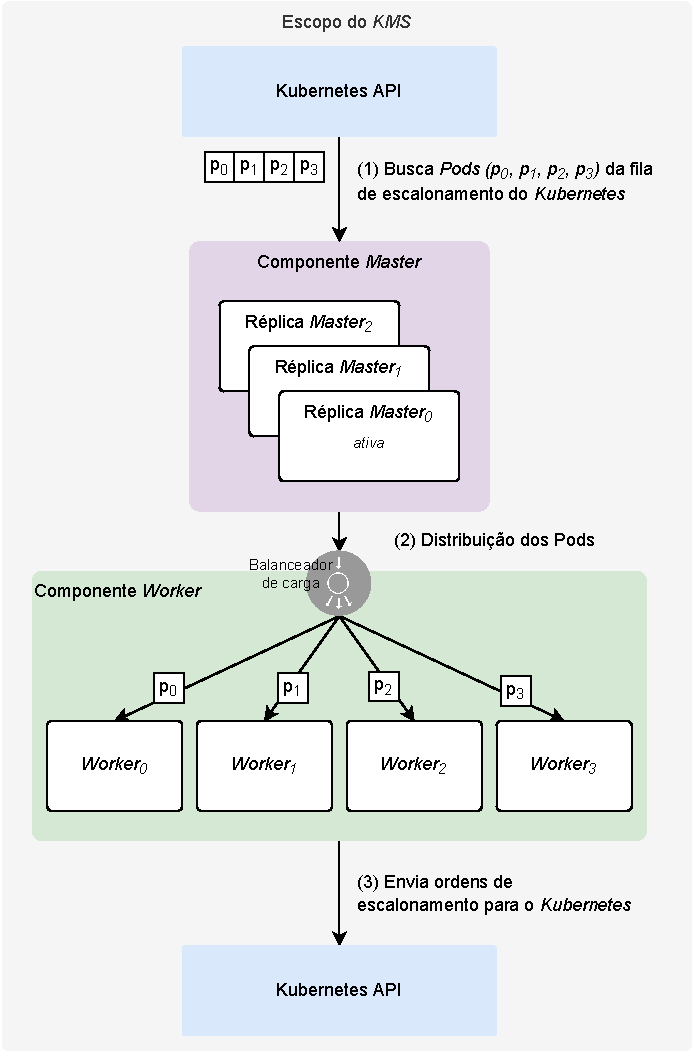
\includegraphics[width=.60\linewidth]{assets/relacao-master-worker.pdf}
	\legend{Fonte: O autor}
\end{figure}

Considerando um cenário do \ac{KMS} com 3 réplicas \textit{Master} e 4 réplicas \textit{Worker}, o funcionamento do sistema distribuído proposto pode ser visualizado na Figura \ref{fig:relacao-master-worker}. O diagrama apresenta a interação completa entre os módulos do \ac{KMS}, desde a coleta do \textit{Pod} pelo \textit{Master}, até o envio da ordem de escalonamento pelo \textit{Worker} para a \textit{API} do \textit{Kubernetes}. Além disso, é possível verificar que no topo do componente \textit{Worker} há um balanceador de carga, que é responsável por distribuir as requisições de escalonamento de \textit{Pods}. Com isso, o componente \textit{Master} não necessita guardar estado das instâncias do \textit{Worker}, uma vez que comunicar-se diretamente com o balanceador de carga é o suficiente. No \textit{Kubernetes} o balanceador de carga pode ser configurado tanto para a estratégia \textit{Binpack} quanto para \textit{Round-Robin}. No exemplo da figura, a estratégia executada foi \textit{Round-Robin}. Outro ponto de destaque são as réplicas do componente \textit{Master}, considerado o \textbf{Produtor} do sistema distribuído, as instâncias do \textit{Master} necessitam executar algoritmo de eleição para manter apenas uma ativa executando a tarefa de \textbf{Produtor}. O algoritmo de eleição será apresentado na Seção \ref{eleicao-master}.

%Na Figura \ref{fig:flow_diagram} é exemplificado o fluxo de execução da arquitetura proposta e os papéis dos dois módulos principais: \textit{master} e \textit{worker}. O \textit{master} é responsável por buscar fila de \textit{pods} não escalonados (1) -- na figura é esboçado por $p_1, p_2, p_3, p_4, p_5, p_6, p_{n-1}, p_n$ -- e também por distribuí-los (2) aos \textit{workers} -- na figura é esboçado por $w_1, w_2, w_{n-1}, w_{n}$ --, nesta etapa foi utilizado o método de espalhamento para enviar a carga de trabalho para os \textit{workers}. Entretanto, o presente trabalho busca modularizar a arquitetura proposta de forma que possibilite intercambiar a técnica de escalonamento e utilizar, por exemplo, agrupamento ou até mesmo métodos refinados. Na etapa (2) será utilizado comunicação via \textit{gRPC}.

%No \textit{worker} há duas funções principais. A primeira é o recebimento das cargas de trabalho como é notado na figura em (2). Para isso cada unidade \textit{worker} gerencia uma fila interna que representa em ordem de chegada as cargas de trabalho enviadas pelo \textit{master}. A segunda função, a principal, é a execução do algoritmo de escalonamento que vinculará o \textit{pod} a um \textit{node}. O método de escalonamento será modular, ou seja, haverá uma lista de implementações de escalonamento pré-definida (\textit{spread, binpack, backfilling}), mas o objetivo é que seja extensível e possa executar até métodos refinados de escalonamento.

\section{Trocas de Mensagens}

A comunicação entre o sistema distribuído proposto e o \textit{Kubernetes} é efetuada pelo protocolo \ac{HTTP}. Em resumo, o \textit{Kubernetes} expõe um servidor \textit{Web} que pode ser consumido por qualquer componente interno. No contexto do presente trabalho, o \textit{Master} consumirá a \textit{API} para buscar os contêineres que estão na fila de escalonamento. Na mesma linha de pensamento, o componente \textit{Worker} se comunicará com a \textit{API} para enviar ordens de escalonamento. A comunicação entre o componente \textit{Master} e \textit{Worker} também será efetivada via protocolo \ac{HTTP}, em síntese, cada instância do \textit{Worker} abrirá um servidor \textit{Web} para consumir as cargas de trabalho enviadas pelo \textit{Master}. Ao utilizar essa arquitetura, é possível definir novas rotas para o servidor \textit{Web} do \textit{Worker}, além daquelas relacionadas ao escalonamento, como por exemplo, rotas para verificar sobrecarga de recursos do contêiner (\textit{CPU} e \textit{RAM}). Para elucidar as trocas de mensagens, foi elaborado um diagrama de sequência com os eventos principais do \ac{KMS} na Figura \ref{fig:sequencia}. 

\begin{figure}[h!]
	\caption{\label{fig:sequencia}Diagrama de Sequência \ac{KMS}}
	\centering
	% \includegraphics[width=0.3\linewidth]{figuras/schedule-proposal.png}
	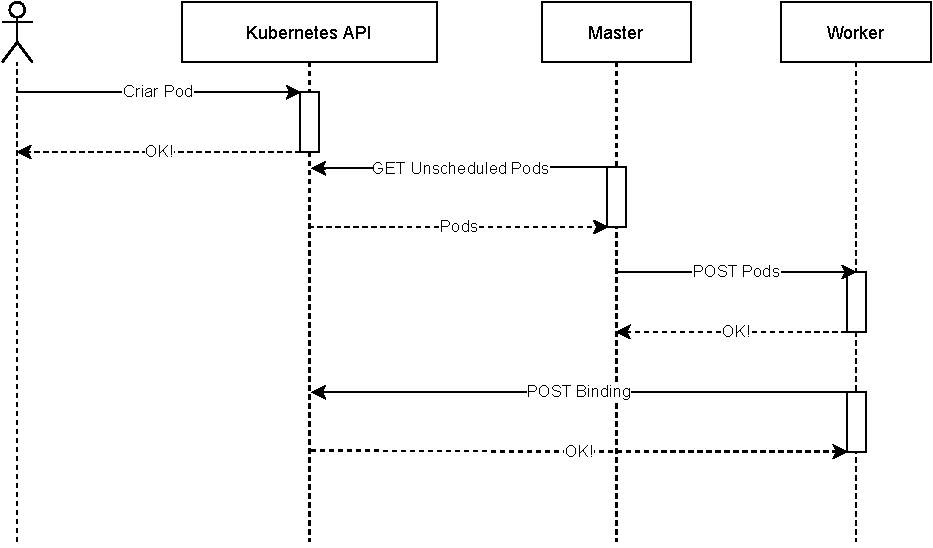
\includegraphics[width=\linewidth]{assets/sequencia.pdf}
	\legend{Fonte: O autor}
\end{figure}

Como todos os módulos do \ac{KMS} se comunicam por \textit{HTTP}, o diagrama de sequência foi elaborado utilizando a nomenclatura padrão de requisições \textit{Web} - \textit{POST e GET}. O ponto de partida é no momento em que um novo \textit{Pod} é inserido na plataforma pelo usuário, devendo ser executado obrigatoriamente pela \textit{API} do \textit{Kubernetes}, na figura corresponde ao evento \textit{Criar Pod}. O \textit{Pod} permanecerá na fila de escalonamento interna até algum escalonador requisitar os \textit{Pods} não escalonados, que é observado no evento \textit{GET Unscheduled Pods}. O próximo passo é distribuir os \textit{Pods} para os \textit{Workers} por meio do evento \textit{POST Pods}, que é executado pelo \textit{Master}. Ao fim, o \textit{Worker} executa o escalonamento e envia uma ordem do tipo \textit{binding} para a \textit{API} do \textit{Kubernetes}, que vinculará o \textit{Pod} à algum nó eleito pelo \textit{Worker} no processo de escalonamento. Essa última etapa é representada pelo evento \textit{POST binding}.


\section{Eleição do Componente \textit{Master} \label{eleicao-master}}

Um dos princípios do \ac{KMS} é desenvolver uma aplicação distribuída sem um único ponto de falha. Essa abordagem influencia que todos os módulos do sistema necessitem alguma técnica de controle de falhas. As instâncias do \textit{Worker} são considerados microsserviços e todas as sua réplicas trabalham simultaneamente no escalonamento. Entretanto, o módulo \textit{Master}, mencionado nas seções anteriores como \textbf{Produtor} do sistema distribuído, demanda que apenas uma réplica esteja ativa trabalhando no escalonamento enquanto que as outras estarão em espera. Dado o contexto, verificou-se que uma das formas de resolver este problema é utilizar algoritmo de eleição para manter apenas uma instância do \textit{Master} executando o escalonamento enquanto que o restante permanecerão em estado de espera.

Visando simplificar o desenvolvimento, as réplicas do componente \textit{Master} se comunicarão com o \textit{Redis} \cite{Redis} para executar o ambiente de eleição. Ao contrário da abordagem padrão de banco de dados relacionais, o \textit{Redis} é considerado não relacional do tipo Chave-Valor em memória. A principal utilização dessa tecnologia é no \textit{caching} de informação devido ao seu rápido acesso aos dados. Além disso, é possível utilizar com persistência em disco, transmissão em tempo real de informação (\textit{Streaming Engine}) e mensagens de inscrição em tópicos do tipo \textit{Publish/Subscribe}, em conclusão, o \textit{Redis} é uma eficiente tecnologia no desenvolvimento de sistemas distribuídos.

O principal objetivo da escolha do \textit{Redis} é se beneficiar da funcionalidade de \textit{Locks Distribuídos}. Os \textit{Locks Distribuídos} são considerados uma primitiva de banco de dados, que auxiliam em cenários nos quais diferentes processos operam recursos compartilhados de forma mutuamente exclusiva \cite{redisDistributedLocks}.

\subsection{Algoritmo de eleição apoiado no \textit{Redis}}

Em síntese, o processo de eleição, baseado em \textit{Locks Distribuídos}, consiste em reproduzir um cenário de corrida entre os processos, o primeiro que conseguir escrever a sua identificação no recurso compartilhado do \textit{Redis} será eleito líder. O recurso compartilhado é no formato de um campo Chave-Valor e possui tempo de expiração (\textit{TTL - Time to live}), o campo voltará a ser nulo no momento em que atingir a data de expiração, dessa forma, habilitando uma nova corrida entre os processos.

Para exemplificar a execução do algoritmo de eleição apoiado no \textit{Redis}, foi desenvolvido um diagrama com 6 passos. Neste exemplo, considere que há 3 réplicas do componente \textit{Master} que estarão disputando a eleição do líder. A réplica que for eleita executará o escalonamento e as regras do \textit{Master}, enquanto que as restantes permanecerão em espera por uma nova oportunidade de eleição. Os diagramas podem ser vistos na Figura \ref{fig:eleicao-todos-os-passos}.

\begin{figure}[h!]
	\caption{\label{fig:eleicao-todos-os-passos}Processos de eleição do \textit{Master}}
	\centering
	% \includegraphics[width=0.3\linewidth]{figuras/schedule-proposal.png}
	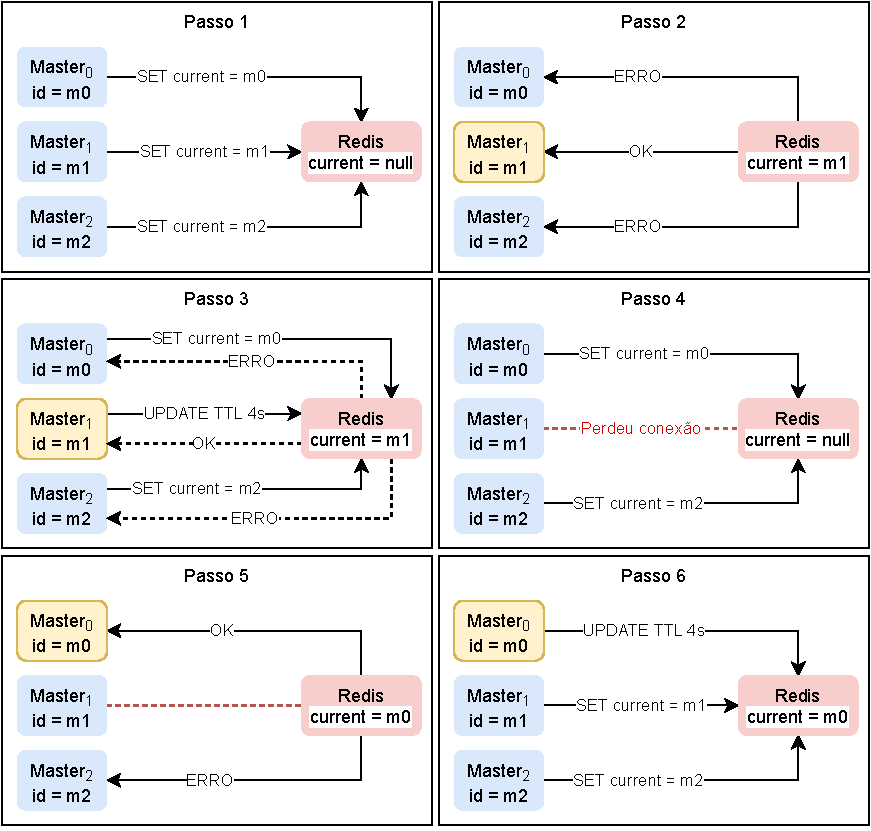
\includegraphics[width=\linewidth]{assets/eleicao-todos-os-passos.pdf}
	\legend{Fonte: O autor}
\end{figure}

\subparagraph{Passo 1:} Todos os \textit{Masters} tentarão escrever no campo \textit{current} do Redis o próprio \textit{id}. Por exemplo, \textit{Master$_2$} tentará escrever \textit{m2} em \textit{current}. O campo \textit{current} foi configurado para ser compartilhado de forma mutuamente exclusiva e possui tempo de expiração de 4 segundos.

\subparagraph{Passo 2:} \textit{Redis} vai utilizar \textit{lock} interno e apenas uma instância do \textit{Master} conseguirá escrever o id no campo \textit{current}. Só é possível escrever se o campo current for nulo. Nesse exemplo, \textit{Master$_1$} foi premiado e tornou-se líder. Neste passo, o \textit{Redis} responde com sucesso apenas o \textit{Master$_1$}.

\subparagraph{Passo 3:} O \textit{Redis} está configurado para expirar o campo \textit{current} a cada 4 segundos, assim permitindo a corrida entre os \textit{Masters}.
Ao passo que, o líder, no caso \textit{Master$_1$}, a cada intervalo de 2 segundos estenderá o \textit{TTL} do campo \textit{current} em 4 segundos.

\subparagraph{Passo 4:} Considere que o \textit{Master$_1$} perdeu a conexão ou foi derrubado. Ou seja, não irá conseguir atualizar o \textit{TTL} do valor \textit{current}. Portanto, em 4 segundos o valor \textit{current} voltará a ser nulo, dessa forma, habilitando uma nova corrida entre os \textit{Masters}.

\subparagraph{Passo 5:} Como o campo \textit{current} voltou a ser nulo, uma nova corrida é executada. Considere que o \textit{Master$_0$} conseguiu escrever \textit{m1} em \textit{current} e será o novo líder e responsável por atualizar o \textit{TTL} enquanto ainda estiver disponível.

\subparagraph{Passo 6:} Este passo representa o reinício do algoritmo, em que o último líder eleito, no caso o \textit{Master$_0$}, será responsável por atualizar o \textit{TTL} do campo \textit{current}. No momento em que não for possível atualizar, o campo voltará a ser nulo dando início uma nova corrida entre as réplicas.


\section{Implantação em \textit{Kubernetes}}
O \ac{KMS} é executado no topo do \textit{Kubernetes}, dessa forma, os componentes principais são conteinerizados e provisionados pelo próprio \textit{Kubernetes}. Na Seção 2.2.4 foram apresentadas 4 formas distintas de customizar o escalonador padrão, após analisar a viabilidade, chegou-se a conclusão que o método \textbf{Múltiplos escalonadores} é o ideal para a implementação do projeto. Essa abordagem consiste no desenvolvimento de um escalonador que é executado no formato de \textit{Pod} e toda a comunicação com o \textit{Kubernetes} é realizada via troca de mensagens por meio da \textit{API}. Com isso, o componente \textit{Worker} é considerado \textit{stateless}, pois as suas dependências (estado do \textit{cluster} e a lista de \textit{Pods} não escalonados) são considerados parâmetros. Neste contexto, o problema de escalonamento, na visão do \textit{Worker}, é da forma entrada e saída: a entrada é o estado do \textit{cluster} que é informado pela \textit{API}, a saída é a ação de escalonamento efetuada pelo \textit{Worker}. Portanto, o escalonador proposto será executado ao lado do escalonador padrão e representado por um conjunto de \textit{pods}. A Figura \ref{fig:proposta_kubernetes} demonstra um caso de uso com 2 instâncias de \textit{Workers} que coordenam o escalonamento de 4 \textit{Nodes} do \textit{Kubernetes}, o \textit{Worker$_0$} é responsável pelo \textit{Node$_0$} e \textit{Node$_2$} (cor roxa) já o \textit{Worker$_1$} pelo \textit{Node$_1$} e \textit{Node$_3$} (cor amarela).

\begin{figure}[h!]
	\caption{\label{fig:proposta_kubernetes}Exemplo de implantação.}
	\centering
	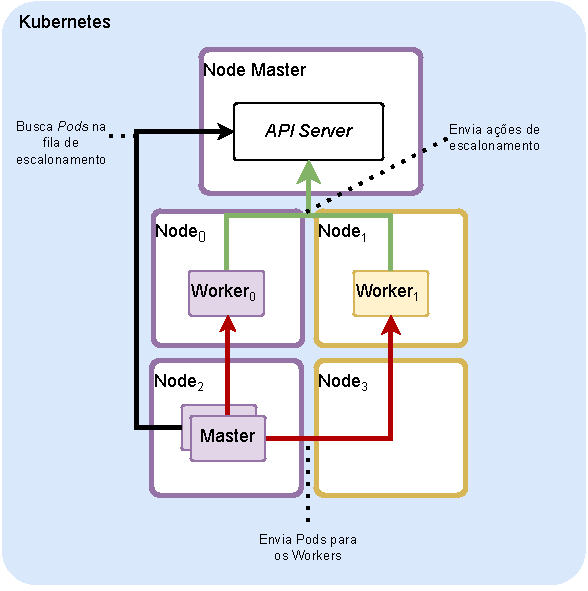
\includegraphics[width=.7\linewidth]{assets/arquitetura-worker.pdf}
	\legend{Fonte: O autor}
\end{figure}

Na figura percebe-se que as instâncias do componente \textit{Master} residem no \textit{Node$_2$}, isso se deve ao fato que as instâncias dos componentes do \ac{KMS} são conteinerizados e escalonadas pelo escalonador padrão do \textit{Kubernetes}. Logo, não é tarefa do escalonador proposto pré definir os nodes em que as próprias instâncias serão executadas, isso é tarefa do \textit{Kubernetes} por meio do escalonador padrão.

Ao utilizar o método de múltiplos escalonadores, no momento de provisionar um novo \textit{pod} para a plataforma é necessário discriminar o escalonador desejado, que é possível por meio do atributo \textit{schedulerName}. Isso é alterado facilmente no arquivo de manifesto do \textit{pod}, como ilustra a Figura \ref{fig:pod_custom_scheduler}.

\begin{figure}[h!]
	\caption{\label{fig:pod_custom_scheduler}Direcionamento do \textit{pod} para o escalonador \textit{my-scheduler}}
	\centering
	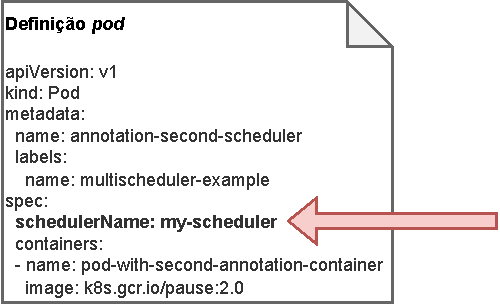
\includegraphics[width=0.6\linewidth]{assets/pod-custom-scheduler.pdf}
	\legend{Fonte: O autor}
\end{figure}

\section{Representação por Diagramas de Classes}

O diagrama de classes da proposta é visualizado pelas figuras \ref{fig:master_class_diagram} e \ref{fig:worker_class_diagram}. No diagrama do \textit{Worker} é utilizado o padrão de projeto \textit{strategy} para alternar o método de escalonamento, além disso, há também outros dois métodos -- \textit{solve} e \textit{binding}. \textit{Solve} é responsável por resolver o escalonamento de acordo com a estratégia escolhida, e \textit{binding} tem como objetivo enviar uma ordem de escalonamento para \textit{Kubernetes} utilizando a \textit{API}.

\subsection{Master}
\begin{figure}[h!]
	\caption{\label{fig:master_class_diagram}Diagrama de Classes \textit{Master}}
	\centering
	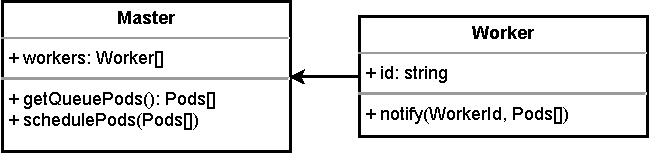
\includegraphics[width=0.65\linewidth]{assets/master-class-diagram.pdf}
	\legend{Fonte: O autor}
\end{figure}

\subparagraph{Classe \textit{Worker}:}
Representa a entidade \textit{Worker} no escopo do \textit{Master}. Em resumo, consiste em um atributo para identificação -- \textit{id} -- e um método para a comunicação de envio dos \textit{Pods} denominado \textit{notify}.

\subparagraph{Classe \textit{Master}:}
Possui uma lista de \textit{Workers} vinculados, é responsável por buscar os \textit{Pods} que estão na fila de escalonamento do \textit{Kubernetes} -- \textit{getQueuePods}. Já o método \textit{schedulePods} objetiva executar o particionamento e direcionar cada parte da fila de escalonamento para um \textit{Worker} específico.
\subsection{Worker}
\begin{figure}[h!]
	\caption{\label{fig:worker_class_diagram}Diagrama de Classes \textit{worker}}
	\centering
	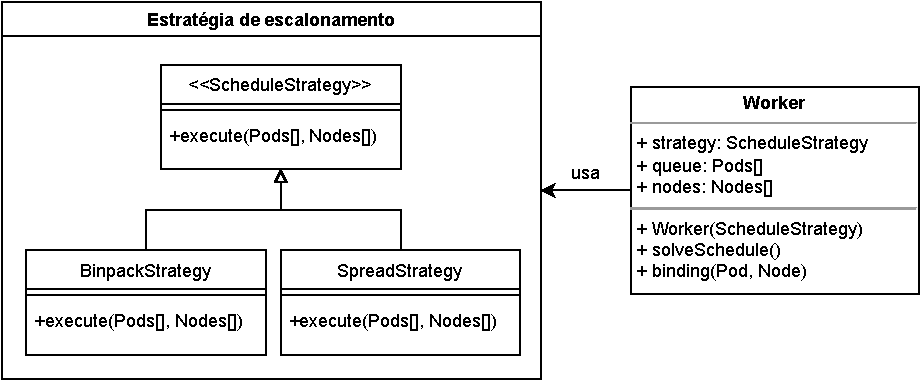
\includegraphics[width=1\linewidth]{assets/worker-class-diagram.pdf}
	\legend{Fonte: O autor}
\end{figure}

\subparagraph{Interface \textit{ScheduleStrategy}:}
Implementação do padrão de projeto \textit{Strategy}, permite intercambiar o método de escalonamento.

\subparagraph{Classe \textit{BinpackStrategy}:}
Executa o escalonamento utilizando técnica de agrupamento.

\subparagraph{Classe \textit{SpreadStrategy}:}
Executa o escalonamento utilizando técnica de espalhamento.

\subparagraph{Classe \textit{Worker}:}
Executa o escalonamento a partir da estratégia selecionada. A estratégia é escolhida no método de construção da classe \textit{Worker(ScheduleStrategy)}. Também há a especificação da fila de escalonamento representado pelo atributo \textit{queue} e dos nós -- \textit{nodes} -- que o \textit{Worker} está gerenciando. O método \textit{solveSchedule} executa o escalonamento a partir da estratégia selecionada e \textit{binding} envia ordem de escalonamento para \textit{API} do \textit{Kubernetes}.

\section{Considerações parciais}
A proposta apresentada nesse capitulo visou o desenvolvimento de um sistema distribuído, fundamentada em microsserviços, para escalonamento de contêineres em \textit{Kubernetes}. Na seção 3.1 foram confrontadas as abordagens de escalonamento oferecidas pelo \textit{Kubernetes} ao lado do \ac{KMS},  a seguir foram levantados os requisitos com objetivo de definir o escopo do projeto. As seções subsequentes explicaram o funcionamento dos componentes principais do \ac{KMS}, com ênfase na característica \textit{stateless} do \textit{Worker}. Na seção 3.4 foi demonstrada a troca de mensagens entre os sistemas, e em sequência a explicação do algoritmo de eleição do componente \textit{Master}. Por fim, foi apresentado um exemplo de implantação do \ac{KMS} em \textit{Kubernetes} e a identificação dos diagramas de classes dos componentes principais.
 






% ----------------------------------------------------------

% ----------------------------------------------------------
% Plano de testes
% ----------------------------------------------------------
% TODO: TIRAR LEVE DOS TESTES

\chapter{Plano de testes}
Esse capítulo visa apresentar o plano de testes utilizado no ambiente de execução deste trabalho de conclusão de curso. A primeira seção descreve a infraestrutura virtual e também as configurações do \textit{cluster} \textit{Kubernetes} utilizadas nos testes. Em seguida, são apontados os parâmetros aplicados no ambiente de testes e as métricas de interesse coletadas. Na Seção 4.3 é apresentado o simulador de eventos responsável pelas execuções dos testes em diferentes cenários de erros de escalonamento. Por fim, as considerações parciais são apresentadas.

%Um dos principais desafios do presente trabalho é investigar e definir os parâmetros da arquitetura proposta. A princípio, há dois parâmetros inicias os quais serão desenvolvidos: (1) variação no número de réplicas do escalonador e (2) quantidade de \textit{nodes} do \textit{cluster} que cada \textit{worker} gerenciará. No contexto do presente trabalho, (1) será variado em diversas rodadas de testes, será considerado de início apenas 2 réplicas e subir a quantidade gradativamente até atingir o limite físico da arquitetura. Já (2) possui um nível de complexidade maior que (1), a forma natural é dividir de forma proporcional, por exemplo, em um \textit{cluster} com 10 \textit{nodes} e 5 \textit{workers} então cada \textit{worker} gerenciará 2 \textit{nodes}. Contudo, de acordo com a literatura, esse é um parâmetro que há margem de refinamento. Considera-se o trabalho de \citeonline{vaucher2018sgxaware}, o qual consiste em escalonamento em \textit{cluster} heterogêneo -- máquinas com diferentes arquiteturas e capacidades de processamento. Neste cenário, não seria interessante utilizar o método proporcional de divisão entre \textit{workers} e \textit{nodes}. Outro exemplo é o trabalho de \citeonline{Wang2019Pigeon}, o qual consiste em particionar o \textit{cluster} de acordo com a complexidade das cargas de trabalho. Este trabalho sugere que cargas de trabalho menores devem ser executadas em um segmento do \textit{cluster} diferente que cargas de trabalhos consideradas complexas. Neste cenário houve acréscimo do desempenho na métrica de tempo de espera.

%As métricas de interesse do presente trabalho estão relacionadas com o desempenho de escalonamento em cenários de falhas. Quanto menos tempo uma carga de trabalho permanecer na fila, maior é o desempenho da proposta de escalonamento. Portanto, há duas métricas que serão avaliadas de acordos com os parâmetros propostos: tempo de espera de escalonamento e \textit{makespan}. As métricas de sobrecarga também serão importantes, principalmente relacionadas a sobrecarga do \textit{node}, seja de espaço ou processamento.

\section{Infraestrutura Virtual}
O ambiente de testes foi cedido pela nuvem computacional privada da UDESC em ambiente virtualizado \textit{OpeStack}. Ao todo, possui 20 \textit{vCPUs} e 40 \textit{GB} de memória \textit{RAM}. A partir dos recursos disponíveis foram provisionadas 9 máquinas virtuais \textit{Ubuntu Cloud 20.04 LTS}, para  a construção de um \textit{cluster} \textit{Kubernetes} na versão 1.23.5. As configurações das máquinas do \textit{cluster} são denominadas \textit{m1.medium} (2 \textit{vCPUs} e 4 \textit{GB} de memória \textit{RAM}) e \textit{m1.large} (4 \textit{vCPUs} e 8 \textit{GB} de memória). O \textit{cluster} provisionado possui  2 nós responsáveis pelo \textit{Control Plane} com o objetivo de trabalhar com alta disponibilidade, sendo o nó principal com a configuração \textit{m1.large} e o nó réplica representado por uma instância \textit{m1.medium}. Além disso, há mais 6 máquinas \textit{m1.medium}, sendo 6 nós trabalhadores do \textit{cluster} \textit{Kubernetes} e uma máquina responsável pelo balanceador de carga do \textit{Kube API Server}. A visualização do \textit{cluster} configurado, representado por um conjunto de máquinas virtuais, pode ser visualizado na Figura \ref{fig:openstack}.
\begin{figure}[h!]
	\caption{\label{fig:openstack}Implantação no \textit{OpenStack}}
	\centering
	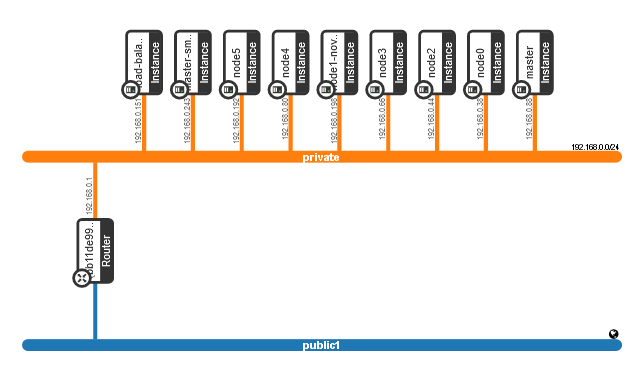
\includegraphics[width=.7\linewidth]{assets/openstack.png}
	\legend{Fonte: O autor}
\end{figure}

\section{Parâmetros e Métricas}
Um dos principais desafios na construção do ambiente experimental é a investigação e as definições de parâmetros e métricas de interesse. Os parâmetros estão relacionados com o ambiente de testes, sendo eles: quantidade total de \textit{pods} submetidos a plataforma (50), quantidade total de simulações de \textit{crashes} de escalonamento (varia de acordo com o cenário de erro que será posteriormente apresentado) e tempo de espera do evento de submissão de \textit{pods} (6 segundos). Este último parâmetro será esclarecido na Seção \ref{sec-simulador-de-eventos}. Já os parâmetros relacionados ao sistema de escalonamento são: quantidade de réplicas do escalonador padrão configurado em alta disponibilidade (1) e quantidade de réplicas dos componentes \textit{Master} (3) e \textit{Worker} (3) do \ac{KMS}.

As métricas de interesse do presente trabalho estão relacionadas com o desempenho de escalonamento em cenários de falhas. Quanto menos tempo uma carga de trabalho permanecer na fila, maior é o desempenho da proposta de escalonamento. Portanto, há duas métricas que serão avaliadas no ambiente de testes de acordos com os parâmetros propostos: tempo de espera de escalonamento e \textit{makespan}.

\section{Simulador de eventos \label{sec-simulador-de-eventos}}
Para analisar as abordagens de escalonamento foi desenvolvido um simulador de eventos discretos com o intuito de exercitar o escalonador. O simulador de eventos possui como parâmetros o total de \textit{pods} que são enviados à plataforma e quantidade total de eventos e erros de escalonamento. As cargas são enviadas para a plataforma de forma gradual respeitando a curva de distribuição normal, com o objetivo de simular um ambiente de produção. No contexto desse simulador, um evento de submissão corresponde a uma quantidade $n$ de \textit{pods} que serão enviados para a plataforma de forma assíncrona, isto é, todos os \textit{pods} de um evento são enviados simultaneamente ao escalonador. Além de enviar \textit{pods}, o simulador também é responsável por simular erros nos sistemas de escalonamento. O erro faz com que o escalonador não esteja disponível por um período de tempo, consequentemente, quanto maior o tempo que o escalonador permanecer indisponível maior será a degradação das métricas de desempenho. 

%Portanto, a técnica de recuperação de falhas e a eficiência da eleição são os pontos determinantes do escalonamento em cenário de falhas.

Os testes realizados consistem em enviar um total de 120 \textit{pods} ao escalonador propagados em 50 eventos de submissões, sendo que cada evento possui duração de 6 segundos e são executados de forma síncrona. Isto é, um evento inicia sua execução apenas após o término da execução do evento anterior. Os \textit{pods} submetidos à plataforma foram construídos para estressar o consumo de memória, visto que mensurar uma alocação válida de \textit{CPU} é um processo complexo por se tratar de um valor excepcionalmente volátil. Logo, as foram definidos como requisitos de recursos computacionais $128$\textit{MiB} de memória \textit{RAM} sem uma  quantidade mínima de \textit{vCPU}. O gráfico que representa o modelo padrão dos testes é exibido na Figura \ref{fig:workload-distribution}.

% Em um cenário ideal as métricas de escalonamento de um \textit{Pod} representam aproximadamente: \textit{wait time} de $2,5s$, \textit{makespan} de $28s$ e tempo de execução de $25s$. A cada teste são submetidos 100 \textit{pods} e representam uma requisição de recursos totais de $12,8 GB$ de memória e $25,0$ de tempo de ${vCPU}$

\begin{figure}[h!]
	\caption{\label{fig:workload-distribution} Gráfico de submissões}
	\centering
	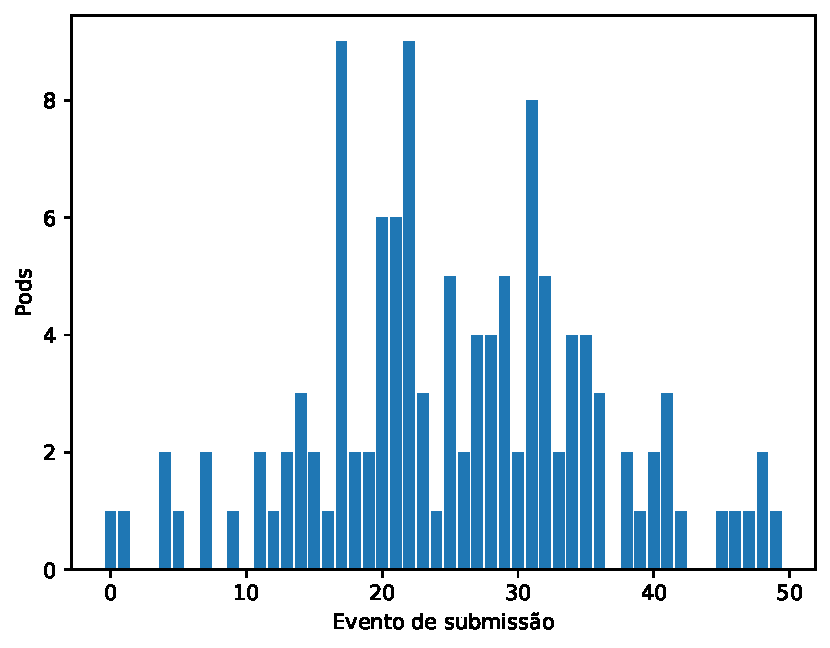
\includegraphics[width=.9\linewidth]{assets/workload-distribution.pdf}
	\legend{Fonte: O autor}
\end{figure}

O simulador de eventos também é responsável por injetar falhas do tipo \textit{crash} ao escalonador em execução. No \textit{Kubernetes}, todos os sistemas internos são representados por \textit{pods} (inclusive o \textit{Kube-Scheduler}), logo, a simulação de uma falha consiste em reinicializar de forma forçada o \textit{pod} responsável pelo escalonamento. Visando observar o comportamento dos escalonadores quando são submetidos a erros, foram desenvolvidos 2 cenários de falhas, denominados Moderado e Intenso. Os cenários de erros visam degradar as métricas de desempenho simulando falhas de escalonamento, no Moderado, ocorreu um disparo total de 5 falhas em eventos estratégicos de submissões de \textit{Pods}, isto é, os eventos 14, 27, 41, 52, 67. No cenário Intenso, há um total de 11 falhas distribuídas nos eventos de submissões 4, 9, 14, 17, 21, 25, 30, 33, 36, 38, 45. 

%O simulador de eventos também é responsável por disparar erros ao escalonador em execução. Uma simulação de erro consiste em derrubar o escalonador em execução, forçando a reinicialização do \textit{pod} que o representa. Serão utilizados 3 cenários de falhas durante as baterias de testes, com o objetivo de analisar as abordagens de escalonamento em diferentes cenários de falhas. Os cenários de falhas, ou \textit{profile}, é um reflexo do modelo padrão dos testes, entretanto, inserindo algumas simulações de falhas em certos eventos de submissão. Os profiles de falhas são denominados de Leve, Moderado e Intenso:
%\begin{enumerate}[label=(\alph*)]
%	\item Leve: 2 disparos de falhas nos eventos 21 e 61;
%	\item Moderado: 4 disparos de falhas, eventos  12, 30, 50 e 67; e
%	\item Intenso: 9 disparos de falhas, eventos 2, 12, 25, 31, 37, 45, 52, 62, 74.
%\end{enumerate}
Os disparos de falhas são executados após o evento de submissão de \textit{pods}. Por exemplo, a falha que está no evento 21 degradará o escalonamento a partir do evento 22. A Figura \ref{fig:profiles-erro} representa cada \textit{profile} sobreposto ao teste padrão de execução, onde as barras em vermelho são as injeções de falhas ao escalonador em execução.

\begin{figure}%
	\centering
	\subfloat[\centering Moderado]{{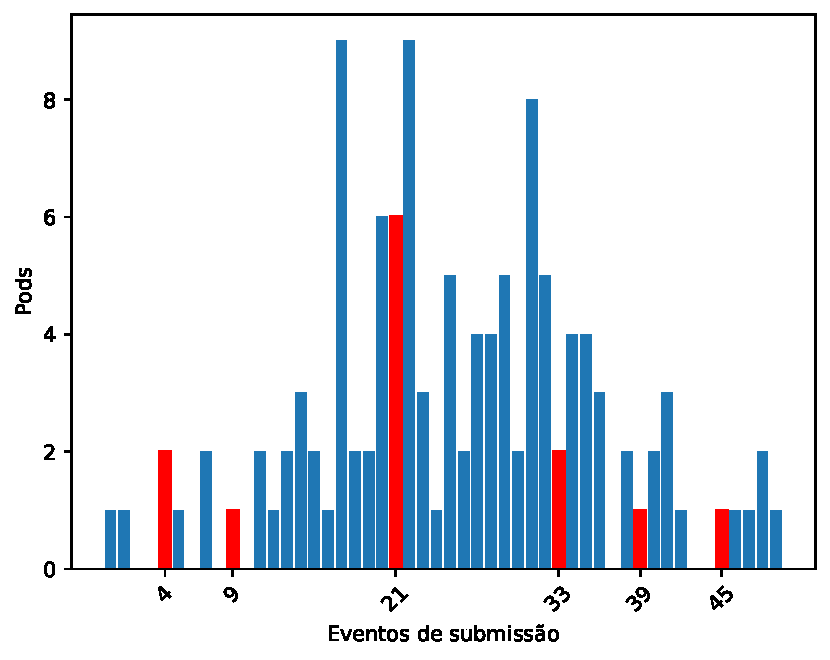
\includegraphics[width=.70\linewidth]{assets/error-moderado.pdf} }}%
	\qquad
	\subfloat[\centering Intenso]{{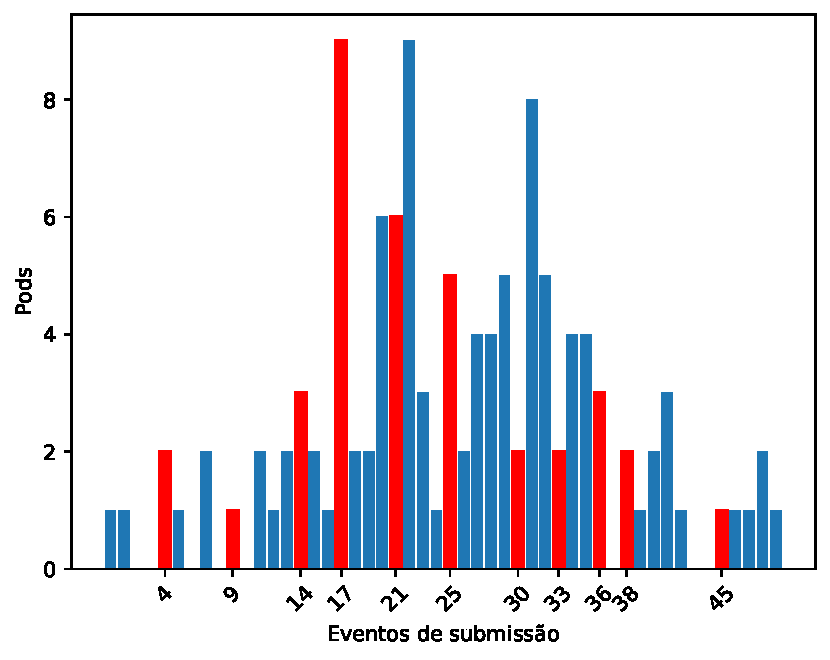
\includegraphics[width=.70\linewidth]{assets/error-intenso.pdf} }}%
	%\qquad
	%\subfloat[\centering Intenso]{{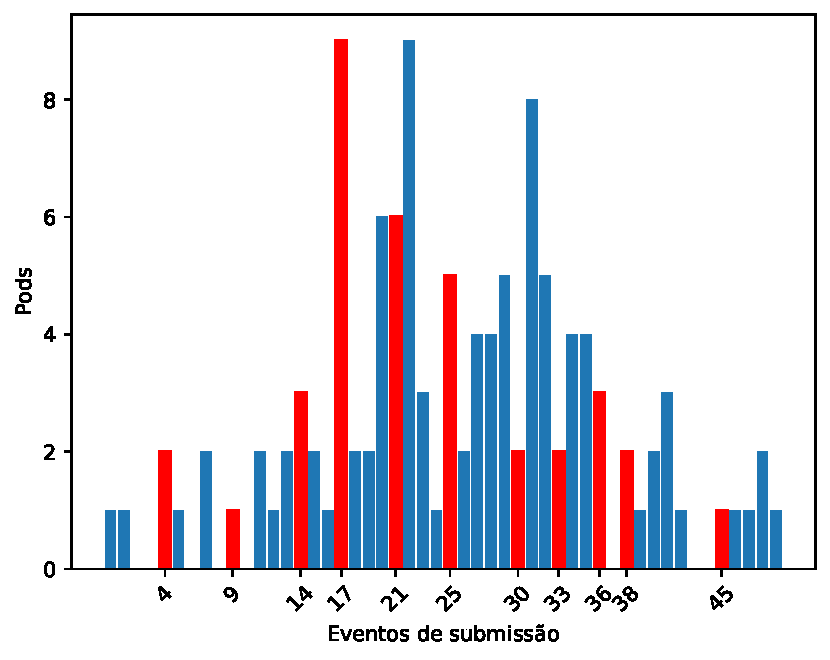
\includegraphics[width=.55\linewidth]{assets/error-intenso.pdf} }}%
	\caption{Cenários de falhas}%
	\label{fig:profiles-erro}%
\end{figure}

\section{Considerações parciais}

O presente capítulo apresentou um protocolo experimental para analisar o desempenho do escalonador proposto.
%
Dois cenários foram elaborados, denominados Moderado e Intenso.
%
Em suma, os cenários variam o número de falhas que ocorrem na infraestrutura computacional.
%
Por definição, as falhas sempre ocorrem em recursos que hospedam partes do escalonador.
%
Os resultados experimentais são apresentados no próximo capítulo, comparando o escalonador proposto no trabalho com as abordagens utilizadas como padrão na arquitetura \textit{Kubernetes} tradicional.
%TODO explicar o algoritmo de simulador de eventos
%TODO pseudocódigo
%TODO definir um profile fixo de disparo de erros
























% ----------------------------------------------------------

% ----------------------------------------------------------
% Plano de testes
% ----------------------------------------------------------
\chapter{Análise de Resultados}
Neste capítulo, os resultados obtidos com a execução dos \textit{profiles} de falhas Moderado e Intenso, que foram apresentadas na Seção 4.3, são apresentados e analisados. Busca-se concluir que há otimização das métricas de desempenho de escalonamento no escalonador proposto em comparação com as abordagens padrão do \textit{Kubernetes} (com e sem réplica) em cenários de falhas. Na Seção 5.1 serão apresentados os resultados para base de comparação, em sequência, nas Seções 5.2 e 5.3 os resultados com interferência das falhas de escalonamento. Para cada análise de cenário, será apresentada uma tabela que representa a média dos valores encontrados nos testes, enquanto os gráficos temporais são baseados na mediana. Além disso, o escalonador padrão será denominado \textit{Padrão}, e a configuração com réplicas de \textit{Padrão*}. O escalonador proposto é denominado de \textit{KMS}. Ao fim do capítulo será feita uma revisão e conclusão dos testes realizados.

\section{Cenário referência}

Esse cenário investigou os valores usados como base de comparação para as métricas de escalonamento sem a interferência de falhas. Portanto, é considerado o valor referência da análise, pois evidenciará a perda de desempenho do escalonamento ao ser comparado com os \textit{profiles} das seções posteriores.

A Figura \ref{fig:cenario-base} representa a composição dos resultados. Na tabela são informadas as médias dos testes executados para cada abordagem de escalonamento, já os gráficos mostram a média cumulativa da métrica analisada. Nos gráficos notou-se que os resultados do \ac{KMS} degradaram em relação as outras abordagens no momento em que é submetida a uma carga maior de escalonamento (segundo 90 em diante). Isso deve-se a sobrecarga da arquitetura baseada em microsserviços, principalmente influenciada pelas trocas de mensagens entre os sistemas. Outro fator a salientar, o \textit{KMS} faz requisições ao \textit{Kube-API} para buscar a lista de \textit{Pods} e enviar ordens de escalonamento, logo está submetido ao tempo de resolução desse serviço. O \textit{Kube-Scheduler} também utiliza a \textit{Kube-API}, entretanto, possui maior prioridade por se tratar de um serviço do \textit{Control Plane}.

 \begin{figure}[!ht]
	\centering
	\begin{tabular}[b]{cccc}\hline
		Escalonador & Tempo Espera & \textit{Makespan} & \textit{Slowdown}\\ \hline
		Padrão  & 2,765s & 38,551s & 1,702\\
		Padrão* & 3,70s  & 43,636s & 1,166 \\
		KMS     & 4,49s & 41,789s & 1,860 \\ \hline
	\end{tabular}
	\qquad
	\subfloat[\centering Média cumulativa do Tempo de espera]{{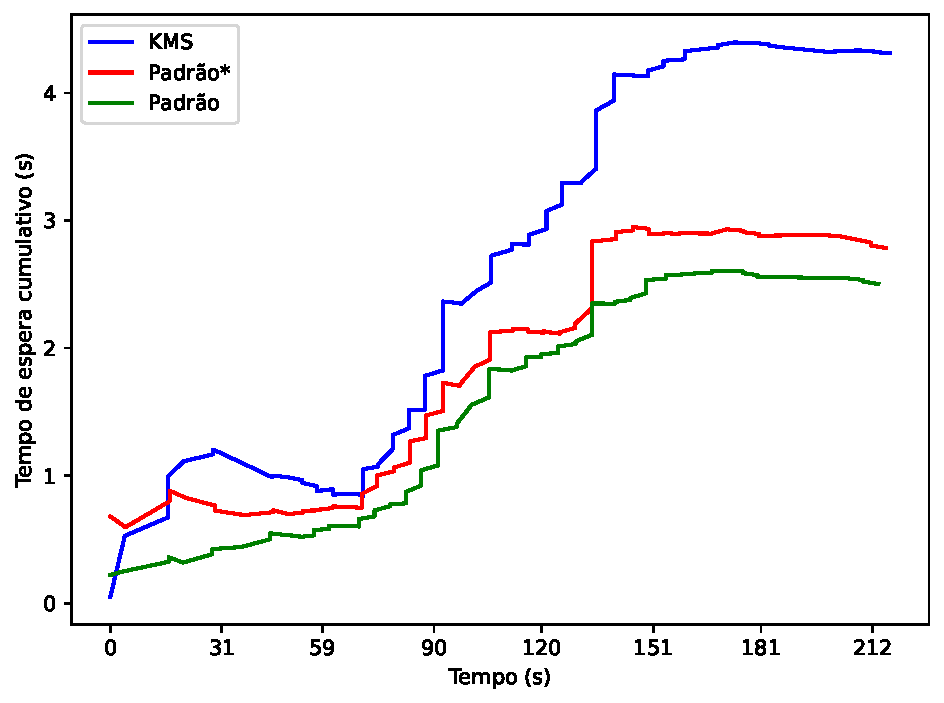
\includegraphics[width=.465\linewidth]{assets/waittime-base.pdf} }}
	\qquad
	\subfloat[\centering Média cumulativa do Makespan]{{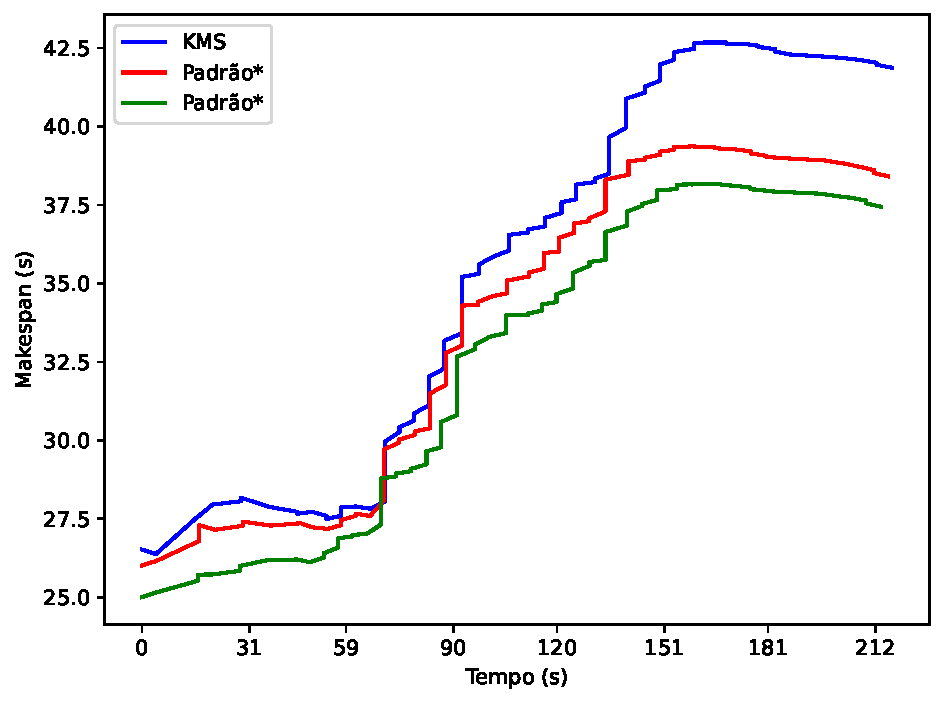
\includegraphics[width=.465\linewidth]{assets/makespan-base.pdf} }}
	\qquad
	\subfloat[\centering Média cumulativa do Slowdown]{{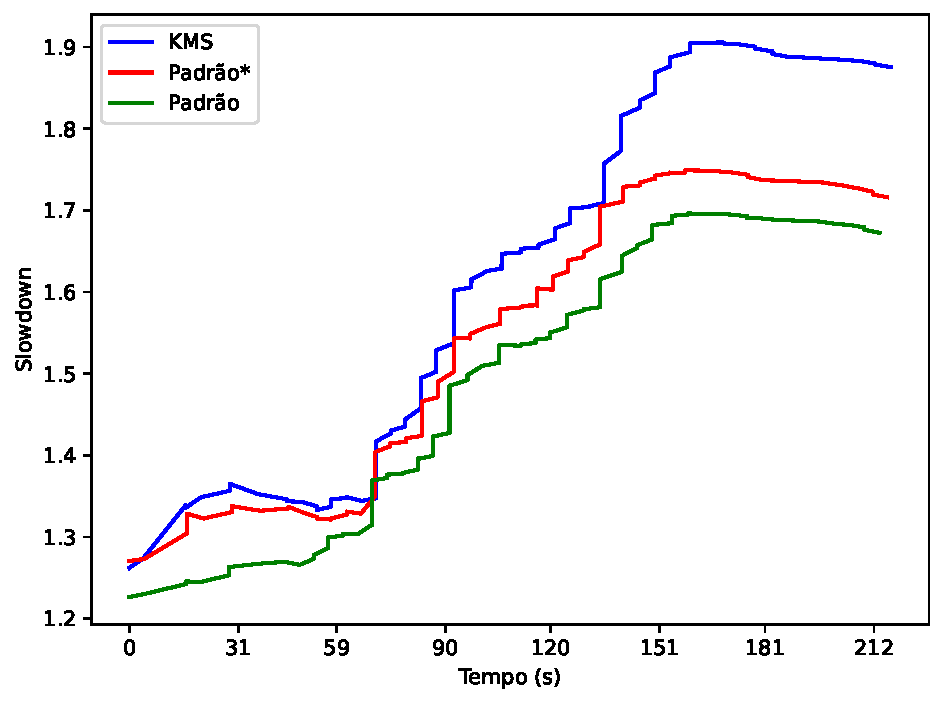
\includegraphics[width=.57\linewidth]{assets/slowdown-base.pdf} }}
	\caption{Composição resultados Referência: Tabela e gráficos de desempenho}
	\label{fig:cenario-base}
\end{figure}

Os gráficos evidenciaram, de forma geral, uma proporção entre os resultados. Esse comportamento era o esperado no cenário base pois não houveram interferência de falhas nem sobrecarga dos recursos computacionais do \textit{cluster}. Nota-se os resultados positivos que a abordagem Padrão apresentou no Tempo de Espera, já o escalonador com réplica resultou em uma ótima taxa de \textit{Slowdown}, evidenciando melhor equilíbrio entre o tempo de espera e escalonamento das cargas de trabalho.


 \newpage
\section{Resultados para o cenário Moderado}
O plano de testes moderado consistiu em submeter os escalonadores às falhas de escalonamento. No total foram 6 simulações de \textit{crashes}, com o objetivo de comprovar que o escalonador padrão degrada as métricas de desempenho, enquanto que o escalonador com réplica e o \textit{KMS} possuem um melhor controle perante falhas.

\begin{figure}[!ht]
	\centering
	\begin{tabular}[b]{cccc}\hline
		Escalonador & Tempo Espera & \textit{Makespan} & \textit{Slowdown}\\ \hline
		Padrão  & 24,84s & 69,57s & 3,13\\
		Padrão* & 8,62s  & 49,71s & 2,178 \\
		KMS     & 4,87s & 43,22s & 1,92 \\ \hline
	\end{tabular}
	\qquad
	\subfloat[\centering Média cumulativa do Tempo de espera]{{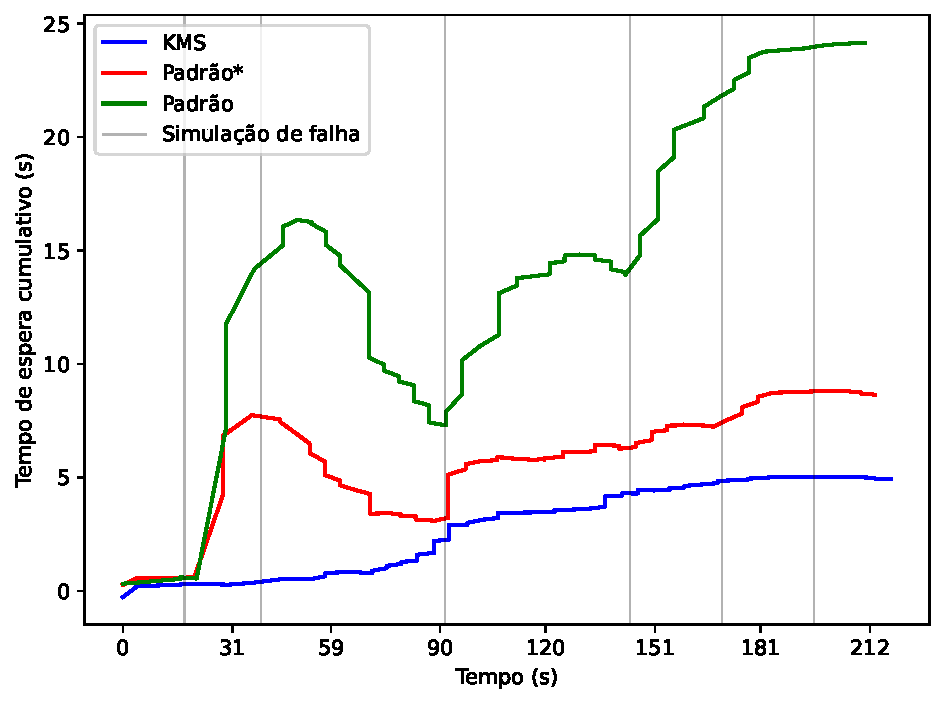
\includegraphics[width=.465\linewidth]{assets/waittime-moderado.pdf} }}
	\qquad
	\subfloat[\centering Média cumulativa do Makespan]{{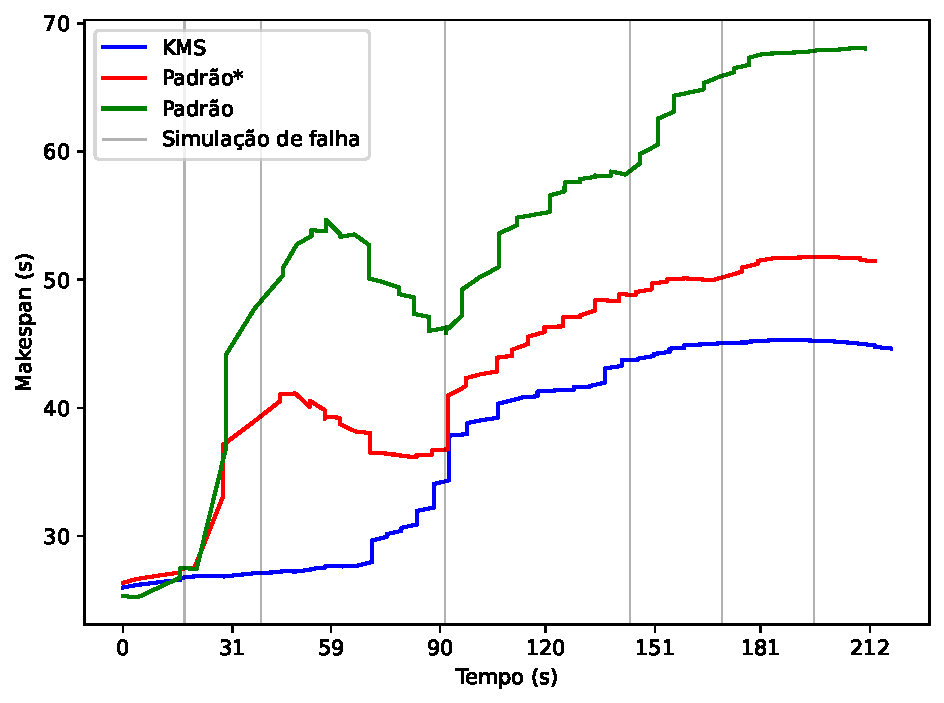
\includegraphics[width=.465\linewidth]{assets/makespan-moderado.pdf} }}
	\qquad
	\subfloat[\centering Média cumulativa do Slowdown]{{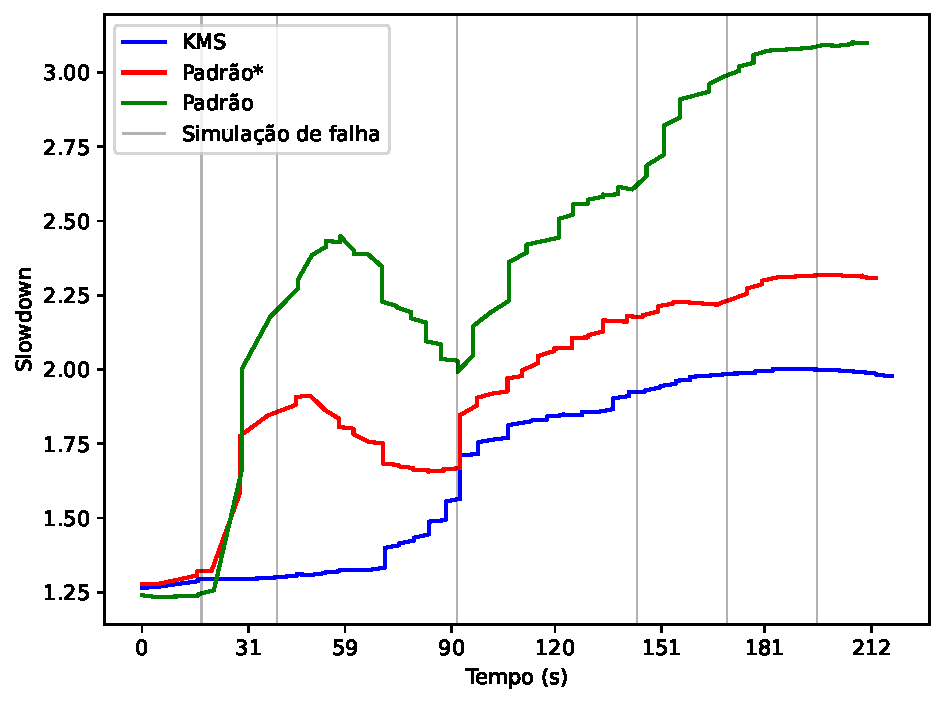
\includegraphics[width=.57\linewidth]{assets/slowdown-moderado.pdf} }}
	\caption{Composição resultados Moderado: Tabela e gráficos de desempenho}
	\label{fig:cenario-base}
\end{figure}

%Neste \textit{profile} obteve-se resultado acima do esperado com o \textit{KMS}, pois o número de falhas era consideravelmente pequeno, entretanto, foi o suficiente para degradar as métricas do escalonador \textit{Padrão} e o \textit{Padrão*}.
Neste \textit{profile} é possível analisar a queda de desempenho das abordagens quando são injetados erros de escalonamento. Embora exista degradação em todas as comparações, como é visto no escalonador \textit{Padrão} que piorou a métrica de tempo de espera em 798\% e o \textit{Padrão*} em 132\%, o \textit{KMS} degradou a métrica de tempo de espera em apenas 8\%. Os dois primeiros são sistemas monolíticos que possuem dependências e inicializações complexas, acarretando em deixar o processo de escalonamento ocioso por certos períodos de tempos. Por sua vez, o \textit{KMS}, quando ocorre alguma falha, apenas uma instância do sistema é derrubada e todas as outras estão ativas resolvendo escalonamento. As falhas no \textit{KMS} influenciaram pouco em comparação com o teste anterior, houve uma variação de apenas 0,38s no tempo de espera, 1,43s de \textit{makespan} e 0,06 de \textit{slowdown}. Nos intervalos [0,90] dos gráficos, nota-se um pico de aumento nas métricas. O escalonador padrão com réplica suportou bem esse pico, isso é evidenciado no tempo 90 em que igualou suas médias cumulativas das métricas com o \ac{KMS}. Entretanto, no decorrer dos testes, foram simuladas mais falhas distanciando as métricas das abordagens apontando o desempenho do \ac{KMS}.

\newpage
\section{Resultados para o cenário Intenso}
Para o \textit{profile} Intenso,  foi configurado uma elevada taxa de falhas durante o período de testes, aumentando o tempo de indisponibilidade do escalonador \textit{Padrão}. Por esse motivo foram desconsiderados os valores dessa abordagem, e a análise considera somente as métricas de escalonamento do \textit{Padrão*} e \textit{KMS}.

\begin{figure}[!ht]
	\centering
	\begin{tabular}[b]{cccc}\hline
		Escalonador & Tempo Espera & \textit{Makespan} & \textit{Slowdown}\\ \hline
		Padrão  & N/C & N/C & N/C\\
		Padrão* & 29,83s  & 78,62s & 3,52 \\
		KMS     & 10,52s & 52,59s & 1,92 \\ \hline
	\end{tabular}
	\qquad
	\subfloat[\centering Média cumulativa do Tempo de espera]{{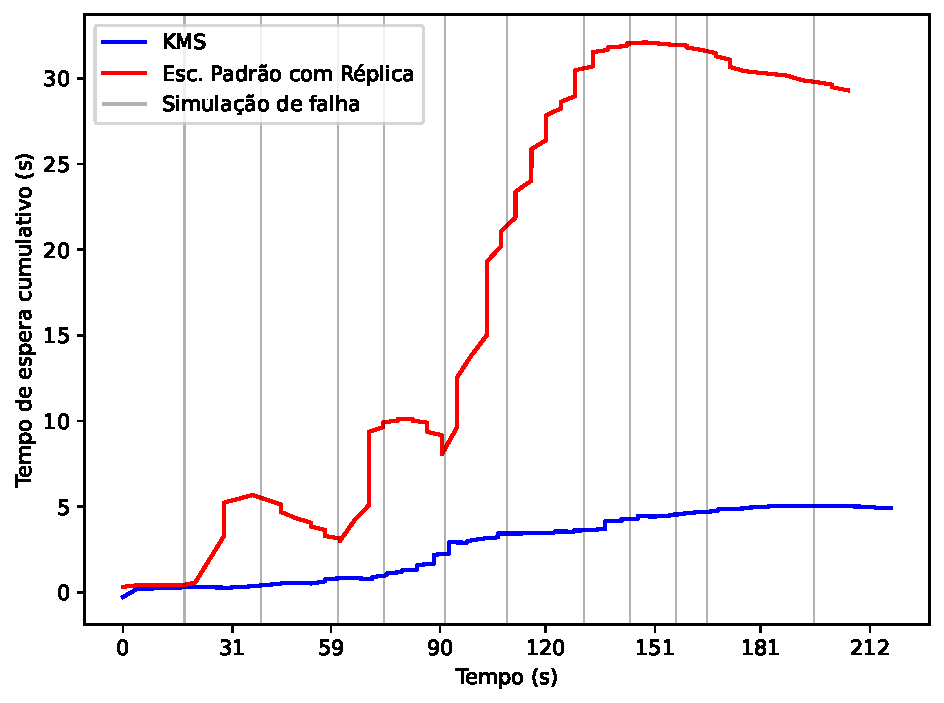
\includegraphics[width=.465\linewidth]{assets/waittime-intenso.pdf} }}
	\qquad
	\subfloat[\centering Média cumulativa do Makespan]{{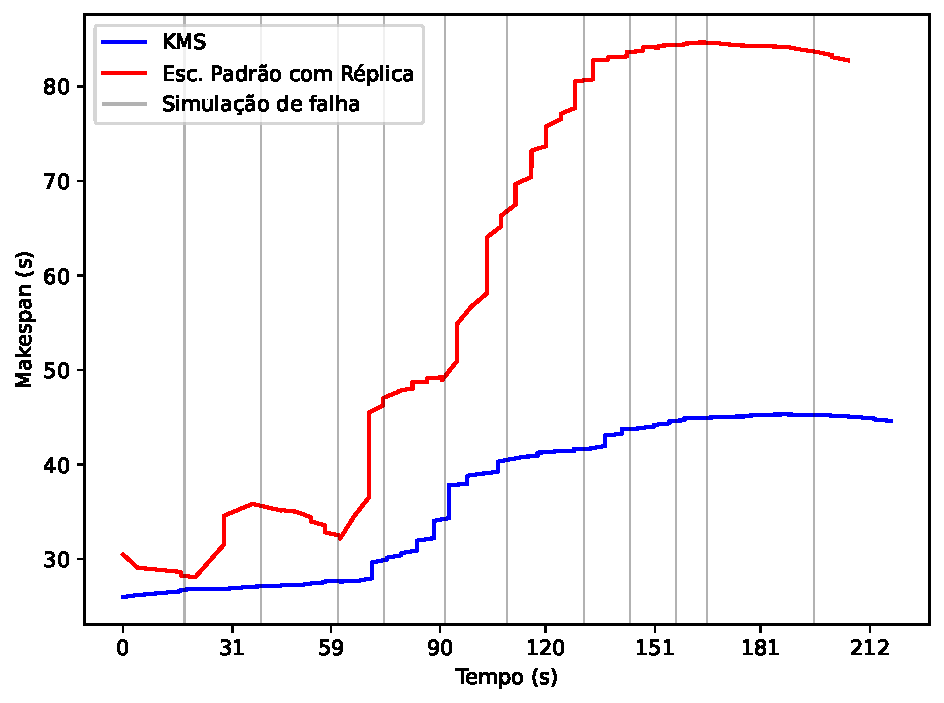
\includegraphics[width=.465\linewidth]{assets/makespan-intenso.pdf} }}
	\qquad
	\subfloat[\centering Média cumulativa do Slowdown]{{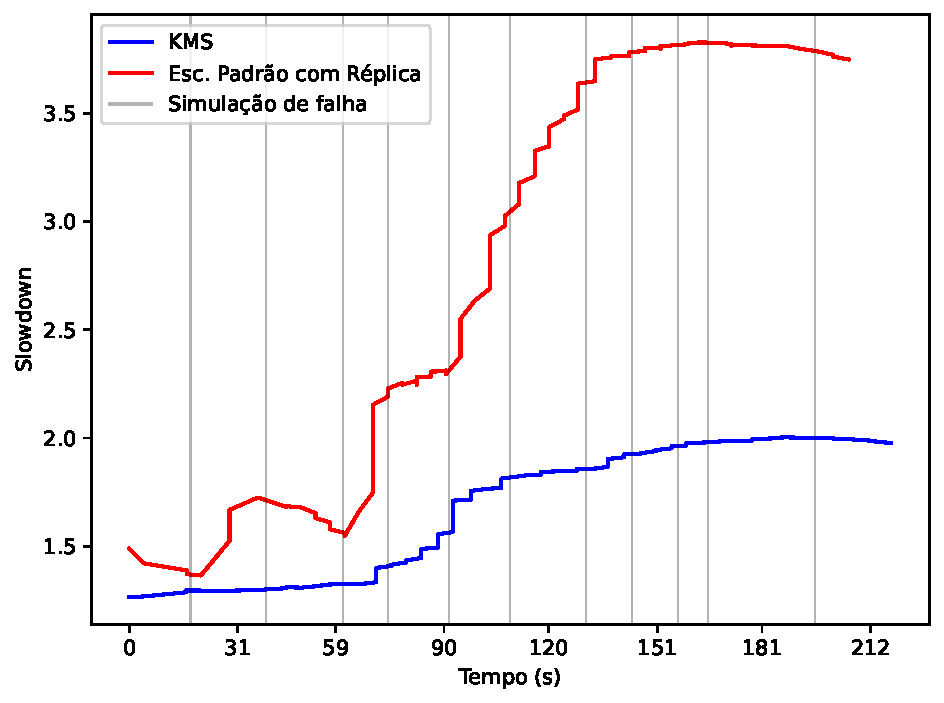
\includegraphics[width=.57\linewidth]{assets/slowdown-intenso.pdf} }}
	\caption{Composição resultados Intenso: Tabela e gráficos de desempenho}
	\label{fig:cenario-intenso}
\end{figure}

O \textit{Profile} Intenso foi desenvolvido para apontar o desempenho do \textit{KMS} quando é submetido a um grande volume de falhas em sequência. A abordagem de réplica do \textit{Kubernetes} é interessante e possui uma ótimo desempenho em cenários moderados, entretanto, em um cenário caótico as métricas são degradadas como comprovam os gráficos da Figura \ref{fig:cenario-intenso}. Possuindo um pico acentuado a partir do tempo 90, enquanto que o \textit{KMS} possui um pico controlado, devido as suas características de sistemas distribuídos e microsserviços.

\section{Considerações parciais}
Os testes executados demonstraram a eficiência do escalonador proposto \ac{KMS} em cenários de falhas. A abordagem \textit{Padrão} do \textit{Kubernetes} foi bem avaliada no cenário referência, enquanto nos cenários Moderado e Intenso, ocorreram degradações consideráveis nas suas métricas de desempenho. Por fim, a abordagem \textit{Padrão*} desempenhou bem no cenário Moderado, evidenciando o ganho de desempenho ao utilizar alta disponibilidade de escalonamento. Já no cenário Intenso, o elevado volume de submissões de falhas nos hospedeiros dos escalonadores resultou no agravamento nos valores das métricas avaliadas.

A Seção 5.1 apontou os valores bases das métricas de escalonamento em um cenário sem falhas. Nesse contexto, o escalonador padrão do \textit{Kubernetes} obteve os melhores resultados em comparação com as outras técnicas abordadas. Essa diferença deve-se a sobrecarga que sistemas distribuídos possuem, principalmente em comunicação. Na seção seguinte, evidenciou-se que um tratamento de falhas é ideal para a disponibilidade do serviço de escalonamento, pois o escalonador proposto possui um desempenho superior em comparação ao escalonador padrão. Por fim, na execução dos testes no cenário Intenso, as métricas de escalonamento foram concebíveis apenas na execução do \textit{KMS}, expondo que um sistema distribuído baseado em microsserviços possui um desempenho não alcançado pelos escalonadores monolíticos.





















% ----------------------------------------------------------

% ----------------------------------------------------------
% Proposta
% ----------------------------------------------------------
\chapter{Conclusão}

O escalonamento é considerado um processo de tomada de decisão que está presente em diversos ramos. No contexto desse trabalho, o objetivo é escalonar contêineres em nós computacionais com recursos computacionais finitos. 
Por se tratar de um problema de classe \textit{NP-difícil}~\cite{ullman1975np}, não há algoritmo escalável que resolva o escalonamento de forma ótima, abrindo espaço para soluções baseadas em heurísticas e implementações de diferentes arquiteturas. Na Seção 2.5, Trabalhos Relacionados, foram discutidos alguns projetos de escalonadores de contêineres, entretanto, nenhum considerou a criação de um sistema distribuído. Logo, o presente trabalho, guiado pelo Capítulo 3, visou o desenvolvimento de um escalonador distribuído em microsserviços e tolerante a falhas. Para isso, o escalonador proposto utilizou técnicas de balanceamento de carga, eleição por meio de \textit{Locks Distribuídos} e utilização da abordagem \textit{stateless} no componente responsável pelo escalonamento.  A abordagem de escalonamento distribuída, até o momento, é a solução adotada por empresas, como \textit{Google} e \textit{Microsoft}, para tratarem grande volumes de requisições de escalonamento~\cite{Wang2019Pigeon, Google2015Borg}. 
Especificamente, \textit{Data Centers} de larga escala necessitam de componentes internos sofisticados e adaptáveis que lidam com o gerenciamento de centenas de milhares de cargas de trabalhos, demandando de alguma técnica de alta disponibilidade, pois um pequeno tempo que o processo de escalonamento não está em execução já o suficiente para degradar uma quantidade elevada de métricas, como visto no Capítulo 4.

No Capítulo 5, Análise de Resultados, foi explorada a eficiência da abordagem de escalonamento proposta neste trabalho. No contexto dos testes, foram desenvolvidos 3 cenários diferentes para comparar os escalonadores do \textit{Kubernetes} e o \ac{KMS}. Nos dois últimos cenários, Moderado e Intenso, o escalonador proposto desempenhou como o esperado, lidando bem com o escalonamento mesmo em situação com intenso volume de falhas, não permitindo que os erros degradassem as métricas de desempenho, como aconteceu com os escalonadores padrões do \textit{Kubernetes}.

Portanto, a explosão da demanda de poder computacional dos \textit{Data Centers} fazem com que as Nuvens Computacionais necessitem de sistemas complexos de gerenciamento para manter um bom nível de \textit{QoS} de suas plataformas. Dessa forma, este trabalho desenvolveu um escalonador distribuído baseado em microsserviços, que, amparado pelos resultados em cenários de falhas, se enquadra como uma boa alternativa para alta disponibilidade de escalonamento no \textit{Kubernetes}.

\section{Trabalhos futuros}
\begin{itemize}
	\item Para evitar problemas de consistência cada \textit{Worker} é responsável por uma partição disjunta dos nós disponíveis. Sugere-se como melhoria de implementação, no momento em que uma réplica do \textit{Worker} encontrasse indisponível os seus nós sejam adotados pelo restante das réplicas dos \textit{Workers} remanescentes;
	\item Investigar o impacto das chamadas \textit{HTTP} nas trocas de mensagens entre o \textit{Master} e o \textit{Worker};
	\item Encontrar o nível de ruptura das abordagens de escalonamento em cenário de falhas. Este número pode ser encontrado aumentando gradativamente a quantidade de falhas até que o escalonador em análise permaneça indisponível;
	\item Reescrever a implementação em linguagem compilada, isso diminuirá o tempo de criação da imagem dos contêineres do escalonador proposto, logo, diminuição das métricas em cenário de falhas; e
	\item Reescrever a implementação para utilizar protocolo de troca de mensagem mais leve que o \textit{HTTP}.
\end{itemize}


%este trabalho visou o desenvolvimento de um escalonador distribuído, baseado em microsserviços,
%a principal vantagem dessa abordagem é em cenários de falhas. Em que um escalonador monolítico há a perda total do evento de escalonamento, enquanto que o escalonador deste trabalho há perda somente parcial, pois é um conjunto de serviços que 
%A explosão da demanda de poder computacional dos \textit{data centers} uniram, ainda mais, as áreas entre escalonamento e sistemas distribuídos. O objetivo desse trabalho, é, a partir da interseção entre as duas áreas, propor uma solução distribuída de escalonamento resiliente em cenários de falhas. De acordo com a literatura, \textit{data centers} de larga escala necessitam de componentes internos sofisticados e adaptáveis que lidam com o gerenciamento de centenas de milhares de cargas de trabalho. Assim, a construção de uma arquitetura de escalonamento distribuída, até o momento, é a solução para que as empresas, como \textit{Google} e \textit{Microsoft}, tratem um grande volume de requisições de escalonamento \cite{Wang2019Pigeon, Google2015Borg}.
%Ao unir as áreas entre sistemas distribuídos e escalonamento encontra-se quantidade significativa de estudos explorados, entretanto, a intersecção entre essas áreas junto com orquestradores de contêineres é escasso na literatura como visto no Capítulo 3. Este trabalho possui como objetivo suprir essa carência, uma vez que a principal arquitetura de escalonamento encontrada em \textit{data centers} de larga escala, atualmente, é distribuída.

% ----------------------------------------------------------

% ----------------------------------------------------------
% ELEMENTOS PÓS-TEXTUAIS
% ----------------------------------------------------------
\postextual
% ----------------------------------------------------------

% ----------------------------------------------------------
% Referências bibliográficas
% ----------------------------------------------------------
\bibliography{ref}

%---------------------------------------------------------------------
% INDICE REMISSIVO
%---------------------------------------------------------------------
\phantompart
\printindex
%---------------------------------------------------------------------

\end{document}
